\documentclass[12pt,a4paper,reqno]{article}
\usepackage[left=12mm,top=1.5in,bottom=1.5in,right=12mm]{geometry}
\usepackage{amsmath}
\usepackage{amssymb}
\usepackage{amsmath}
\usepackage{amsthm}
\usepackage[square, comma]{natbib}
\usepackage{comment}
\usepackage{tikz}
\usepackage{float}
\usepackage{todonotes}
\usepackage{bm}
\usepackage{subcaption}
\usepackage{./slashbox}
\usepackage{enumitem}
\setlist{
  listparindent=\parindent,
  parsep=0pt,
  listparindent = 1em
}

\usetikzlibrary{matrix}

\renewcommand{\figurename}{\textsc{Figure}}
\renewcommand{\tablename}{\textsc{Table}}

\usepackage{geometry, color, graphicx, mathtools}

\usepackage{fancyhdr}
\setlength\parindent{0pt}

\pagestyle{fancy}
\fancyhf{}
\rhead{Ria Szeredi, Kenneth Young, Lotte Romijn}
\lhead{MAST90098 Project}
\cfoot{\thepage}

\renewcommand{\baselinestretch}{1.2}


\begin{document}
\title{\textsc{MAST90098 \\ Approximation Algorithms and Heuristics \\ Project - 2016}}
\author{Ria Szeredi, Kenneth Young, Lotte Romijn}
\maketitle


\noindent\fbox{%
    \parbox{\textwidth}{%
\textbf{Makespan Scheduling Problem (MS)} \\

Schedule $n$ jobs with designated processing times on $m$ identical machines in such a way that the whole processing time is minimised. \\

\textbf{Input}:

Positive integers $p_1,p_2,...,p_n$ and an integer $m \geq 2$ for some $n \in \mathbb{N} - \{0\}$. Each $p_i$ is the processing time of the $i$th job on any of the $m$ available machines. \\

\textbf{Constraints}:

For every input instance $(p_1,...,p_n,m)$ of MS, \\ $\mathcal{M}(p_1,...,p_n,m) = $  $\{S_1,S_2,...,S_m \> | \> S_i \subseteq \{1,2,...,n\} \textnormal{ for } i=1,...,m, \> \cup_{k=1}^m S_k = \{1,2,...,n\}, \textnormal{ and }$ \\ $S_i \cap S_j = \emptyset \textnormal{ for } i \neq j \}$. \\

\textbf{Cost}:

For each $(S_1,...,S_m) \in \mathcal{M}(p_1,...,p_n,m)$, \\ $\textnormal{cost}((S_1,...,S_m),(p_1,...,p_n,m)) = \textnormal{max} \{ \sum_{l \in S_i} p_l | i = 1,...,m \}$. \\

\textbf{Goal}:

\textit{minimum}


}
}
\newpage

\section{Greedy Local Search Algorithm for MS} \label{sec:GLS}
We implement a greedy local search (GLS) algorithm for MS, which picks the lowest cost neighbour at any iteration.\\

\section*{1.a. $k$-jump-neighbourhood}

We consider a \textit{k-jump}-neighbourhood: \\

We define a mapping $f_X: \mathcal{M}(x) \rightarrow 2^{\mathcal{M}(x)}$, such that if $\beta = \{\beta_1,\beta_2,...,\beta_m \} \in f_x(\alpha)$ for some $\alpha = \{\alpha_1,\alpha_2,...,\alpha_m \} \in \mathcal{M}(x)$ if $\beta$ can be obtained from $\alpha$ by $k$ ``jumps". \\

Each jump allows some job $p \in S_i$ for some $i \in \{1,...,m\}$ to move to any one of the $m$ machines, including to the one in which it is contained. Hence, after one jump we have one of two cases:
\begin{itemize}
\item $\alpha_i \neq \beta_i$ and $\alpha_j \neq \beta_j$ for some $i \in \{1,...,m\}$ and $j \in \{1,...,m\}$, and $\alpha_\ell = \beta_\ell$ for $\ell \neq i$ and $\ell \neq j$, if job $p$ jumps from machine $i$ to machine $j$; or
\item $\alpha = \beta$ if the job jumps to its own machine.
\end{itemize}

We thus define a ``$k$-jump'' as a sequence of $k$ successive jumps, noting that as job can jump more than once. \\

We can check that the conditions for a suitable neighbourhood are satisfied. Let $\alpha = \{\alpha_1,...,\alpha_m\}$ be an initial, feasible solution.
\begin{enumerate}

\item (\textit{Reflexivity}): Since we allow a job to jump to the machine in which it is already contained, it is possible that, after $k$ jumps, all jobs are in their original machines, and the solution is identical to $\alpha$. Hence, we have that $\alpha \in f_X(\alpha)$ for every $\alpha \in \mathcal{M}(x)$. (We call this a `loop').

\item (\textit{Symmetry}): If $\beta \in f_X(\alpha)$ for some $\alpha \in \mathcal{M}(x)$, then $\alpha \in f_X(\beta)$, since reversing the $k$ jumps from which $\beta$ was obtained from $\alpha$ is also a $k$ jump.

\item (\textit{Connectivity}): If we have any two feasible solutions $\alpha$ and $\beta$, we can always obtain one from the other by performing a finite number of $k$ jumps (since we allow a job to jump to any machine). If $k \geq n$, one $k$-jump suffices, since we allow loops. If $k \leq n$, we perform maximally $\lceil \frac{n}{k} \rceil$ $k$ jumps. Hence, for all $\alpha, \beta \in \mathcal{M}(x)$, there exists a positive integer $k$ and $\gamma_1,...,\gamma_k \in \mathcal{M}(x)$ such that $\gamma_1 \in f_X(\alpha)$, $\gamma_{i+1} \in f_X(\gamma_i)$ for $i=1,...,k-1$, and $\beta \in f_X(\gamma_k)$.

\end{enumerate}

The cardinality of this neighbourhood is quite large. If $k=1$, we can move from one feasible solution of MS to another by moving one job, to the same or a different machine. If we have $n$ jobs and $m$ machines, there are $n \> m$ possible $1$-jumps. For general $k$, there are $(n \> m)^k$ possible $k$-jumps.


\begin{comment}
We also consider a \textit{swap}-neighbourhood: \\

We define a mapping $f_X: \mathcal{M}(x) \rightarrow 2^{\mathcal{M}(x)}$, such that if $\beta = \{\beta_1,\beta_2,...,\beta_m \} \in f_x(\alpha)$ for some $\alpha = \{\alpha_1,\alpha_2,...,\alpha_m \} \in \mathcal{M}(x)$ if $\beta$ can be obtained from $\alpha$ by $k$ swaps. \\

Each swap allows a pair of jobs $(i,j) \in \{1,...,n\} \times \{1,...,n\}$ to swap from machine.

Hence, after one swap $(\alpha_i, \alpha_j) \neq (\beta_i,\beta_j)$ for some $(i,j) \in \{1,...,n\} \times \{1,...,n\}$, and $\alpha_k = \beta_k$ for $k \neq i$ and $k \neq j$.  \\

We can check that the conditions for a suitable neighbourhood are satisfied. Let $\alpha = \{\alpha_1,...,\alpha_m\}$ be an initial, feasible solution.
\begin{enumerate}

\item (\textit{Reflexivity}): Since we allow the swapping of two jobs from the same machine, it is possible that, after a number of $k$-swaps, all jobs are in their original machines, and the solution is identical to $\alpha$. Hence, we have that $\alpha \in f_X(\alpha)$ for every $\alpha \in \mathcal{M}(x)$. (We call this a `loop').

\item (\textit{Symmetry}): If $\beta \in f_X(\alpha)$ for some $\alpha \in \mathcal{M}(x)$, then $\alpha \in f_X(\beta)$, since reversing the $k$ swap from which $\beta$ was obtained from $\alpha$ is also a $k$ swap.

\item (\textit{Connectivity}): If we have any two feasible solutions $\alpha$ and $\beta$, the connectivity property is not always satisfied. For instance, if $\alpha$ and $\beta$ only differ from each other by one job, i.e. one job is positioned into a different machine, then we can not get $\beta$ from $\alpha$ by doing one swap (or a $k$ swap, since we have reflexivity).

\end{enumerate}

Hence, for the \textit{swap}-neighbourhood the connectivity property of a neighbourhood is not satisfied. However, we can consider a neighbourhood which includes both jumps and swaps. In order to do this, we need to determine the order of jumping and swapping. For instance, a $k$-jump followed by an $l$-swap, or an $l$-swap followed by a $k$-jump, or a $k$-jump followed by an $l$-swap followed by an $s$-jump, etc., for positive integers $k$, $l$, $s$. Because such neighbourhoods include the $k$-jump neighbourhood, for which connectivity is satisfied, we have that connectivity is also satisfied for any of these combinations.
\end{comment}


\section*{1.b Implementation} \label{sec:implementation}
We implement the \textit{greedy local search} algorithm in Python (See \emph{GLS} in MS\_heuristics.py). We will call the resulting total processing time, produced by the algorithm, the `makespan value'. \\

In our code for GLS, Variable-Depth Search (Section \ref{sec:VDS}) and Simulated Annealing (Section \ref{sec:simulatedannealing}), we represent a feasible solution $\{S_1,S_2,...,S_m\}$ to the Makespan Scheduling problem as a list $\xi = [\xi_1,\xi_2,...,\xi_n]$ of length $n$, where each $\xi_i \in [1,...,m]$ which represents in which machine job $i$ is contained. Methods have been included which convert the solutions between these two representations (\textit{convertSol\_toListOfMachines} and \textit{convertSol\_toSetsOfJobs}). \\

To find the best $k$-\emph{jump}-neighbour of a solution, we define a function \emph{findBestNeighbour} which returns the best solution that can be reached from the input solution in at most $k$ jumps. It does so by systematically iterating through all possible combinations of jobs to jump and machines to jump to, and updating the solution if a better neighbour is found.\\

The GLS algorithm requires an initial, feasible solution for each instance. We consider two methods do generate initial solutions:
\begin{enumerate}
\item Random: assigning each job to a random machine (see \emph{findInitialFeasibleSolution\_rand}).
\item GMS - Greedy Makespan Scheduling algorithm (see \emph{findInitialFeasibleSolution\_GMS})
\end{enumerate}

The GMS algorithm works by first sorting the jobs by non-increasing processing time, assigning the $m$ largest jobs each to a different machine, and assigning the remaining jobs to the least loaded machine. I.e., using the original problem notation:

\begin{enumerate}
\item We reindex the jobs such that $p_1 \geq p_2 \geq ... \geq p_n$
\item Let $S_i = \{ \}$ for $i=1,...,m$
\item \textbf{For} $i=1,...,m$
\begin{enumerate}
\item $S_i := \{i \}$
\end{enumerate}
\item[] \textbf{end for}
\item \textbf{For} $j=m+1,...,n$ (only if $n > m$)
\begin{enumerate}
\item $M := \textnormal{min} \{ \sum_{l \in S_i} p_l | i = 1,...,m \}$
\item $S_M = S_M \cup \{ j \}$
\end{enumerate}
\item[] \textbf{end for}
\end{enumerate}

We then convert the initial solution $\{S_1,S_2,...,S_m\}$ to the representation $\xi = [\xi_1,\xi_2,...,\xi_n]$ of length $n$, where each $\xi_i \in \{1,...,m\}$ represents in which machine job $i$ is contained, by using \textit{convertSol\_toListOfMachines}, as described before. Both the random and GMS initial solutions are feasible solutions, since all jobs are assigned to one machine $S_i$, such that $\{S_1,S_2,...,S_m \> | \> S_i \subseteq \{1,2,...,n\} \textnormal{ for } i=1,...,m, \> \cup_{k=1}^m S_k = \{1,2,...,n\}, \textnormal{ and } S_i \cap S_j = \emptyset \textnormal{ for } i \neq j \}$. \\

\section*{1.c Selecting the value of $k$} \label{sec:selectingk}
We perform an experimental study on randomly generated instances of MS across a range of $n$ and $m$ values in order to select an appropriate value for $k$. \\

We consider $n=15, 20, 25, 30, 35, 40, 45, 50$, $m=2,4,6,8,10$, and $k=1,2,3$. For each combination of $n$, $m$ and $k$, we generate 1 instance of MS. For each instance, we randomly select the processing times $p_i$, for $i=1,...,n$, uniformly distributed between 1 and 100. We determine the run time of our GLS implementation for each instance, and the solution quality by comparing the makespan value to a lower bound. We define this lower bound to be the least possible makespan value if we were able to process fractions of the jobs on any machine, i.e.
\begin{equation}
\textnormal{lower bound} = \frac{\sum_{i=1}^n p_i}{m}. \label{eq:NaiveLB}
\end{equation}
We subsequently calculate the solution quality, denoting the makespan value produced by GLS as `makespan',
\begin{equation}
\textnormal{`makespan gap'} = \frac{\textnormal{makespan}}{\textnormal{lower bound} - 1} \times 100\%, \label{eq:NaiveMakespanGap}
\end{equation}
which represents the percentage that makespan value is above its lower bound. \\

The results of 1 realisation per $n$, $m$, and $k$, using a random initial solution, are given in Table \ref{tab:Q1c} and Figure \ref{fig:Q1c}.
We show three-dimensional plots of $n$ versus $m$ versus the makespan gap (in percentage) in Figures \ref{fig:Q1cSFig1}, \ref{fig:Q1cSFig3}, and \ref{fig:Q1cSFig5}, and $n$ versus $m$ versus the run time (in seconds) in Figures \ref{fig:Q1cSFig2}, \ref{fig:Q1cSFig4}, and \ref{fig:Q1cSFig6}. For clarity, we only plot values for the makespan between 0 and 20 \%, and values for the run time between 0 and 1200 seconds. We consider a `reasonable' run time to be approximately 20 minutes (1200 seconds). \\

We can see in Tables \ref{tab:Q1ck=1makespangap}, \ref{tab:Q1ck=2makespangap}, and \ref{tab:Q1ck=3makespangap} that in general, the makespan gap decreases for each instance as we increase $k$. The average makespan gap over all $n$ and $m$ values is 6.98\% for $k=1$, 3.68\% for $k=2$, and 1.32\% for $k=3$. Thus, the average makespan gap improves as $k$ increases. For all values of $k$, the makespan gap is larger for small $n$ and large $m$, i.e. when few jobs need to be distributed over many machines. It is especially larger when $n$ is close to $m$. This suggests that our lower bound is not such a great measure of solution quality for these instances. In fact, we know that for the case when $n=m=10$ that the GLS algorithm returns the solution assigning one job to each machine, which cannot be improved upon and thus must be optimal. For any instance when $n$ is close to $m$, the lower bound provides a gross under-estimation of the true optimal; these are the cases when the possibility of each machine having similar total processing time is least likely. This shortcoming lead us to consider other methods of determining solution quality in Section \ref{subsec:SolQual}. \\

In Table  \ref{tab:Q1ck=1runtime}, \ref{tab:Q1ck=2runtime}, and \ref{tab:Q1ck=3runtime}, we see that for all $n$ and $m$, the run time increases as $k$ increases. It increases rapidly: we see that the average run time over all combinations of $n$ and $m$ is 0.072 s for $k=1$, 19.79 s for $k=2$, and 1199 s for $k=3$. As we increase $k$, the size of the neighbourhood increases by a factor of $n \> m$. However, for all combinations of $n$ and $m$, the run time increases by a factor less than $n \> m$ as we increase $k$. Moreover, when $k$ is larger and we increase $n$ and $m$, the neighbourhood increases more (since the size is $(n \> m)^k$). Hence, in the tables we can see that the run time increases faster for larger $k$, as we increase $n$ and $m$. In Figures \ref{fig:Q1cSFig2}, \ref{fig:Q1cSFig4}, and \ref{fig:Q1cSFig6}, the run time has been plotted for $k=1$, $k=2$, $k=3$, respectively. We have used the same range of the run time values (between 0 and 1200 s) for all three plots. Compared to $k=3$, we can see that the run times for $k=1$ and $k=2$ are significantly smaller. However, for $n=50$ and $m=10$, the run time for $k=2$ is approximately 3 minutes (195 seconds), and approximately 500 ($n \> m = 50 \times 10 = 500$) times larger than the run time for $k=1$, which is 0.385 s.   \\

For our remaining experiments, we choose $k=2$. In Figure \ref{fig:Q1cSFig4}, we see that for all instances we have considered so far, the run time is smaller than 20 minutes (1200 seconds). Moreover, the makespan gap is smaller than for $k=1$, for all instances except for $n=15$ and $m=8,10$, i.e. when the number of jobs is relatively close to the number of machines. Hence, we make a trade-off between solution quality and run time, and select $k=2$ as our $k$-value.

\begin{figure}[H]
\begin{center}
{\Large \bf GLS Experiments}
\end{center}
\centering
\begin{subfigure}{.05\textwidth}
\rotatebox[origin=tl]{0}{$k=1$}
\label{fig:Q1cSFig0}
\end{subfigure}
\begin{subfigure}{.45\textwidth}
  \centering
  \tikz[remember picture]\node[inner sep=0pt,outer sep=0pt] (rates1){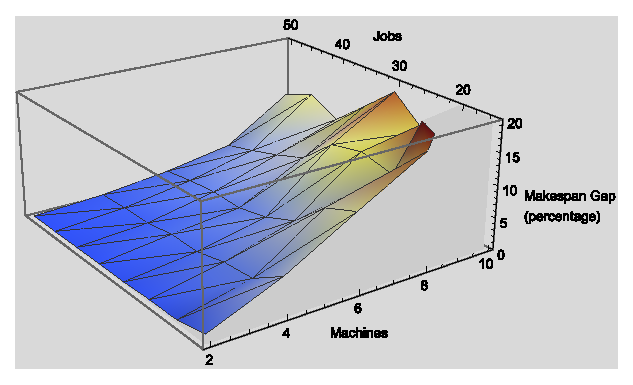
\includegraphics[width=.95\linewidth,height=.7\linewidth]{plots/Q1cRandomMakespangapk=1.eps}};
  \caption{}
  \label{fig:Q1cSFig1}
\end{subfigure}
\begin{subfigure}{.45\textwidth}
  \centering
  \tikz[remember picture]\node[inner sep=0pt,outer sep=0pt] (rates2){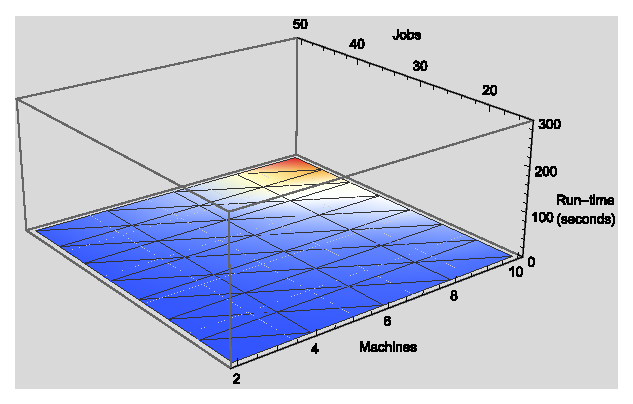
\includegraphics[width=.95\linewidth,height=.7\linewidth]{plots/Q1cRandomRuntimek=1.eps}};
    \caption{}
    \label{fig:Q1cSFig2}
\end{subfigure}
\\
\centering
\begin{subfigure}{.05\textwidth}
\rotatebox[origin=tl]{0}{$k=2$}
\label{fig:Q1cSFig0}
\end{subfigure}
\begin{subfigure}{.45\textwidth}
  \centering
 \tikz[remember picture]\node[inner sep=0pt,outer sep=0pt] (rates3){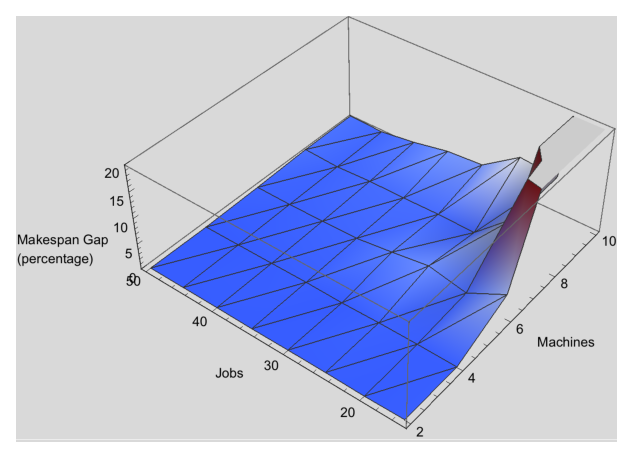
\includegraphics[width=.95\linewidth,height=.7\linewidth]{plots/Q1cRandomMakespangapk=2.eps}};
   \caption{}
  \label{fig:Q1cSFig3}
\end{subfigure}
\begin{subfigure}{.45\textwidth}
  \centering
  \tikz[remember picture]\node[inner sep=0pt,outer sep=0pt] (rates4){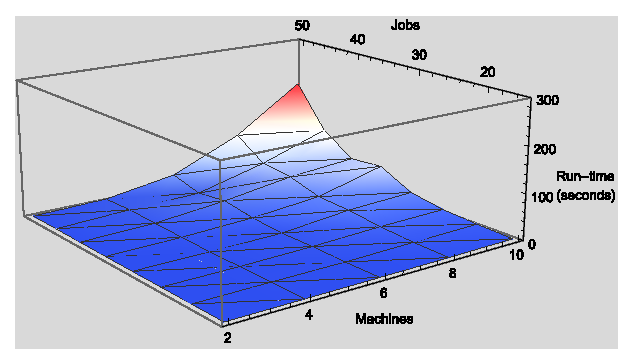
\includegraphics[width=.95\linewidth,height=.7\linewidth]{plots/Q1cRandomRuntimek=2.eps}};
  \caption{}
  \label{fig:Q1cSFig4}
\end{subfigure}
\\
\centering
\begin{subfigure}{.05\textwidth}
\rotatebox[origin=tl]{0}{$k=3$}
\label{fig:Q1cSFig0}
\end{subfigure}
\begin{subfigure}{.45\textwidth}
  \centering
 \tikz[remember picture]\node[inner sep=0pt,outer sep=0pt] (rates3){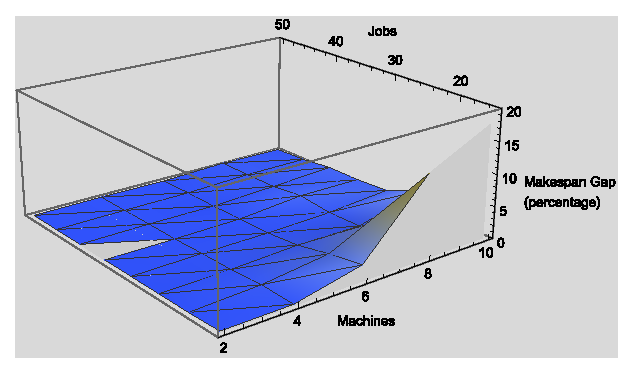
\includegraphics[width=.95\linewidth,height=.7\linewidth]{plots/Q1cRandomMakespangapk=3.eps}};
   \caption{}
  \label{fig:Q1cSFig5}
\end{subfigure}
\begin{subfigure}{.45\textwidth}
  \centering
  \tikz[remember picture]\node[inner sep=0pt,outer sep=0pt] (rates4){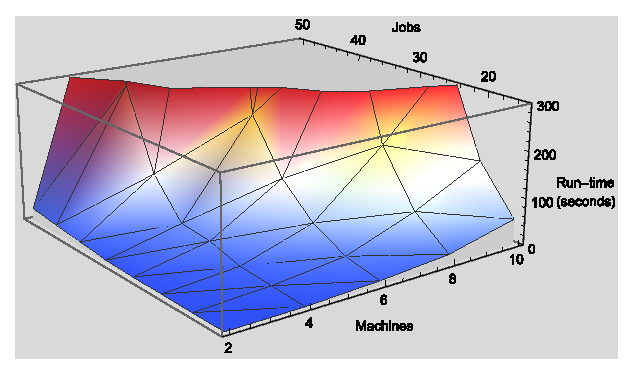
\includegraphics[width=.95\linewidth,height=.7\linewidth]{plots/Q1cRandomRuntimek=3.eps}};
  \caption{}
  \label{fig:Q1cSFig6}
\end{subfigure}
\caption{\textbf{GLS Experiments: $k=1,2,3$, using a random initial solution.}}
\label{fig:Q1c}

\end{figure}

\section*{1.d Experimental Study}
We perform an experimental study to test the performance of the GLS algorithm, using $k=2$. We test for $n=10,20,30,40,50,60,70,80,90,100$ and $m=2,4,6,8,10$. We also now test both methods (random and GMS) for finding an initial feasible solution. \\

For each combination of $n$, $m$ and $k$, we generate 10 instances of MS. For each instance, we randomly select the processing times $p_i$, for $i=1,...,n$, uniformly distributed between 1 and 100. Each instance is generated with a different random seed. \\

We consider a `reasonable' run time to be approximately 20 minutes. The averaged results of 10 realisations per $n$, $m$, and $k$ are presented in Table \ref{tab:Q1d} and Figure \ref{fig:Q1d}. In Figure \ref{fig:Q1d}, only makespan gap values between 0 and 20 \% are plotted, and run time values between 0 and 1200 s (20 minutes). \\

From Table \ref{tab:Q1dmakespangapRandom}, we calculate that the average makespan gap over all $n$ and $m$ for the random initial solution is 4.09 \%. In Table \ref{tab:Q1dmakespangapGMS}, the average makespan gap over all $n$ and $m$ for the GMS initial solution is 4.11 \%. In Table \ref{tab:Q1druntimeRandom}, the average run time over all $n$ and $m$ for the random initial solution is 176.74~s. In Table \ref{tab:Q1druntimeGMS}, the average run time over all $n$ and $m$ for the GMS initial solution is 171.04 s. Hence, the random initial solution and the GMS initial solution give similar results. This suggests that local minima can be found just as easily from either initial solution. We will also use these two methods for generating an initial solution when testing VDS and our heuristic.




\begin{figure}[H]
\begin{center}
{\Large \bf GLS experiments}
\end{center}
\begin{subfigure}{.5\textwidth}
  \centering
  \tikz[remember picture]\node[inner sep=0pt,outer sep=0pt] (rates1){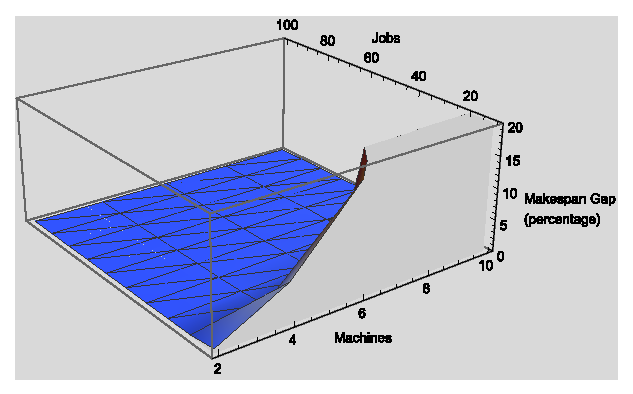
\includegraphics[width=.95\linewidth,height=.7\linewidth]{plots/Q1dRandomMakespanGap.eps}};
  \caption{Random}
  \label{fig:Q1dSFig1}
  \vspace{1cm}
\end{subfigure}%
\begin{subfigure}{.5\textwidth}
  \centering
  \tikz[remember picture]\node[inner sep=0pt,outer sep=0pt] (rates2){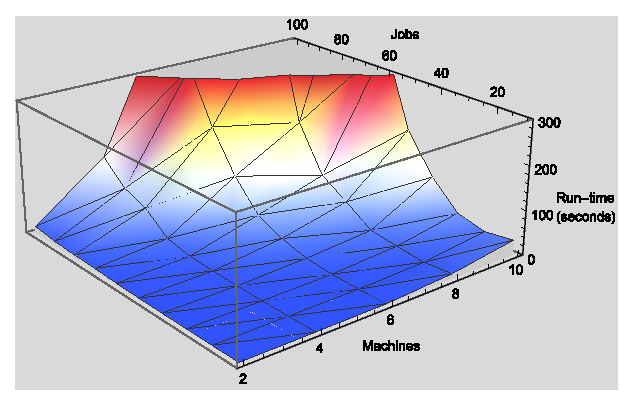
\includegraphics[width=.95\linewidth,height=.7\linewidth]{plots/Q1dRandomRunTime.eps}};
    \caption{Random}
    \label{fig:Q1dSFig2}
    \vspace{1cm}
\end{subfigure}
\begin{subfigure}{.5\textwidth}
  \centering
 \tikz[remember picture]\node[inner sep=0pt,outer sep=0pt] (rates3){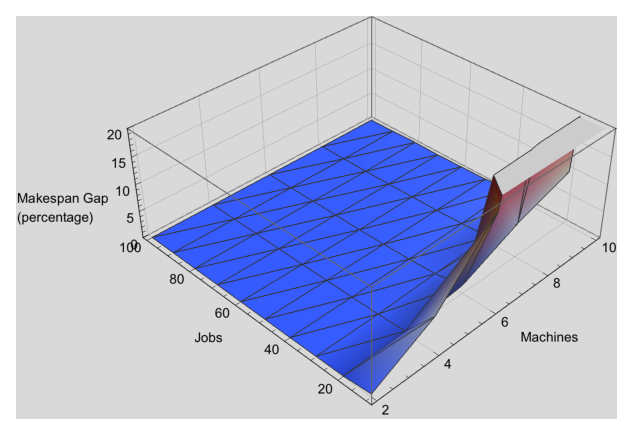
\includegraphics[width=.95\linewidth,height=.7\linewidth]{plots/Q1dGMSMakespanGap.eps}};
   \caption{GMS}
  \label{fig:Q1dSFig3}
\end{subfigure}
\begin{subfigure}{.5\textwidth}
  \centering
  \tikz[remember picture]\node[inner sep=0pt,outer sep=0pt] (rates4){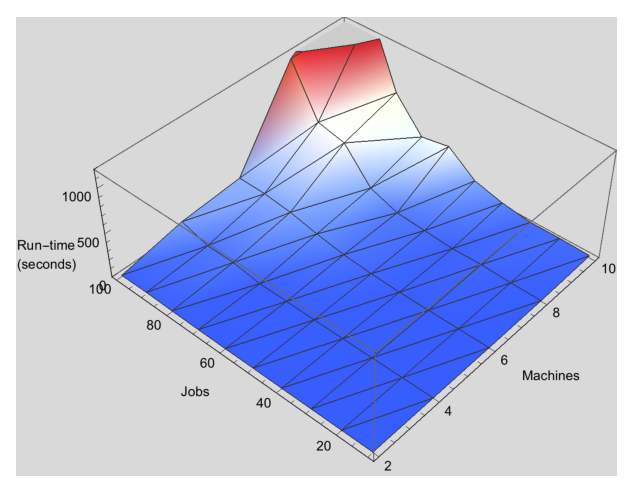
\includegraphics[width=.95\linewidth,height=.7\linewidth]{plots/Q1dGMSRunTime.eps}};
  \caption{GMS}
  \label{fig:Q1dSFig4}
\end{subfigure}
\caption[Experiments GLS: Random and GMS]{\textbf{Experiments GLS: k=2, using random and GMS initial solution.} \small (a) and (b) display the makespan gap (in percentage) and the run time (in seconds), using a random initial solution. (c) and (d) show the makespan gap (in percentage) and the run time (in seconds), using the GMS initial solution. We only plot makespan gap values between 0 and 20 \%, and run time values between 0 and 1200 s. }
\label{fig:Q1d}

\end{figure}










\newpage













\section{Variable Depth Search Algorithm for MS} \label{sec:VDS}

In this section, we consider the Variable-Depth Search (VDS) algorithm. This algorithm searches for an improved solution at a larger distance from the current solution, without performing an exhaustive search of the entire neigbourhood. Doing so gives us a higher chance of escaping local minima. \\

We first present detailed pseudo-code for the VDS, as well as provide a justification that our algorithm satisfies the required conditions. Next, we present the results of an experimental study on the same instances as those used in Section 1(d), and compare the results of the VDS to those of the GLS.

\section*{VDS 2.a}
\textbf{Pseudo-code for VDS}\\
We begin with an input instance $I = (p_1,p_2,...,p_n,m)$ of the Makespan Scheduling problem. Recall that, during implementation, we use a list $\xi = [\xi_1,\xi_2,...,\xi_n]$ of length $n$, to represent a solution.

\begin{enumerate}
\item Generate an initial feasible solution $\xi = \{\xi_1,\xi_2,...,\xi_n\}$ \\ (random or GMS described in Section \ref{sec:implementation})
\item $\textnormal{IMPROVEMENT} := \textnormal{TRUE}$
\item[] $\textnormal{EXCHANGE} := \{1,2,...,n\}$
\item[] $J=0$, $\alpha_J := \xi$
\item \textbf{while} $\textnormal{IMPROVEMENT} = \textnormal{TRUE}$ \textbf{do}
\begin{enumerate}
\item \textbf{while} $\textnormal{EXCHANGE} \neq \emptyset$ \textbf{do}
\begin{enumerate}
\item $J := J+1$
\item $\alpha_J := findBestNeighbour(I,\alpha_{J-1},k,\text{ True, EXCHANGE})$
%the best neighbour in the $k$-neighbourhood of $\alpha_{J-1}$. We define \textit{gain}$(\alpha_{J-1}, \delta) = \textnormal{makespan}(\alpha_{J-1}) - \textnormal{makespan}(\delta)$. Hence, the best neighbour $\alpha_J$ is defined such that \\ \textit{gain}$(\alpha_{J-1},\alpha_J) = $max$\{$\textit{gain}$(\alpha_{J-1},\delta) | \delta \in \textnormal{Neigh}_k(\alpha_{J-1}) - \{\alpha_{J-1} \}$ and $\delta$ differs from $\alpha_{J-1}$ in the parameters of $\textnormal{EXCHANGE}$ only $\}$.
\item $\textnormal{EXCHANGE} := \textnormal{EXCHANGE} - \{\text{jobs whose machines changed in the transition}$\\
\hspace*{6cm} from $\alpha_{J-1} \text{ to } \alpha_{J}\} $
%\item $\textnormal{EXCHANGE} := \textnormal{EXCHANGE} - \{ \textnormal{the parameters in which } \alpha_J \textnormal{ and } \alpha_{J-1} \textnormal{ differ } \}$ (i.e., we remove the job index for which the machine has been changed from $\textnormal{EXCHANGE}$).
\end{enumerate}
\item[] \textbf{end while}
\item Compute \textit{gain}$(\xi,\alpha_i) = \textnormal{makespan}(\xi) - \textnormal{makespan}(\alpha_i)$, for $i=1,...,J$
\item Compute $l \in \{1,...,J\}$ such that \\ \textit{gain}$(\xi,\alpha_l) = \textnormal{max}\{$\textit{gain}$(\xi,\alpha_i) \> | i \in \{1,2,...,J\} \}$
\item \textbf{if} \textit{gain}$(\xi,\alpha_l) > 0$ \textbf{then}
\begin{enumerate}
\item[] $\xi:=\alpha_l$
\item[] $\textnormal{EXCHANGE} := \{1,2,...,n\}$
\item[] \color{red} $J=0$, $\alpha_J := \xi$ \color{black}
\end{enumerate}
\item[] \textbf{else}
\begin{enumerate}
\item[] $\textnormal{IMPROVEMENT} := \textnormal{FALSE}$
\end{enumerate}
\end{enumerate}
\item[] \textbf{end while}
\item \textbf{output}$(\xi)$
\end{enumerate}

\textbf{Neighbourhood function and satisfaction of conditions in Section 3.6.2 of the textbook}

Our neighbourhood function, \textit{findBestNeighbour} (step (3)(a)(ii)), . Finding the best neighbour of a feasible solution, $\alpha_i$ is equivalent to finding a feasible solution, $\alpha_{i+1}$, which is such that $gain(\alpha_i,\alpha_{i+1})=\max\{gain(\alpha_i,\delta) | \delta\in Neigh(\alpha_i)\} = \max\{\textnormal{cost}(\alpha_i) - \textnormal{cost}(\delta) | \delta\in Neigh(\alpha_i)\}$, and we only update $\alpha_i$ to $\alpha_{i+1}$ if $gain(\alpha_i,\alpha_{i+1}) > 0$. Thus condition (ii)(a) in Section 3.6.2 of the textbook is satisfied.\\

In order to satisfy the conditions (i) and (ii)(b), we have included two special input arguments to the \textit{findBestNeighbour} method:
\begin{enumerate}
\item \textit{differentSolRequired} is a Boolean parameter, which indicates whether we require a neighbour which differs by at least one $\xi_i$ to the original solution. This is set to be True for the VDS algorithm (whereas for the GLS algorithm, we set it to False). The function does not update the best neighbour if the neighbour is the same as the input solution. The implementation of this parameter ensures that the final feasible solution has all jobs assigned to a different machine to the original solution. Thus condition (i) is satisfied.
\item \textit{jobsToConsider} is a list representing the jobs whose assigned machine we are allowed to change. The \textit{findBestNeighbour} method only iterates over the jobs in this list in its search for the best neighbour, thus returning a solution which is such that any jobs not in the list stay on their original machine. In the VDS algorithm, the input argument is the EXCHANGE list. Thus, at each iteration within the while loop in step 3.a, we obtain a neighbour which differs from the previous solution in the parameters of EXCHANGE only. This list is initialised as the set of all jobs, and is updated at each iteration of the while loop in step 3.a.iii by removing any jobs that were changed. This procedure is continued until there remain no jobs to be changed, after which we break out of the while loop in step 3.a, and condition (ii)(b) is thus satisfied.
\end{enumerate}

Note that our implementation of the VDS algorithm differs slightly from the textbook. We reset $J$ and $\alpha_J$ in step 3.d, displayed in red, which is not done in the textbook. In subsequent iterations of the while loop (step 3), we do not consider `old' neighbours, i.e. neighbours found by previous iterations of the inner while loop (step 3.a). We chose to do this because these old neighbours can not be better than the current best solution $\xi$, since otherwise we would have moved it before. And by this procedure, we only need to check the value of $J$ gains every iteration of the while loop (step 3), and we terminate if we can not find a better solution among any of the $J$ neighbours generated.

\section*{VDS 2.b}
We use Python to implement the \emph{Variable Depth Search}. See \emph{VDS} in MS\_heuristics.py.

\section*{VDS 2.c}
\subsection*{Experimental results}
We perform an experimental study for VDS using the same instances that were generated for Section 1(d), where we generated 10 instances for each combination of $n$ and $m$. The averaged results are displayed in Table \ref{tab:Q2d} and Figure \ref{fig:Q2c}. \\

From Table \ref{tab:Q2dmakespangapRandom}, we calculate that the average makespan gap over all $n$ and $m$ for the random initial solution is 3.38 \%. In Table \ref{tab:Q2dmakespangapGMS}, the average makespan gap over all $n$ and $m$ for the GMS initial solution is 3.28 \%. In Table \ref{tab:Q2druntimeRandom}, the average run time over all $n$ and $m$ for the random initial solution is 79.30 s. In Table \ref{tab:Q2druntimeGMS}, the average run time over all $n$ and $m$ for the GMS initial solution is 42.69 s. Hence, a local minimum is reached faster from the GMS initial solution than from the random initial solution, but the values of the reached local minima are similar for both initial solution methods. Hence, a best solution is found more easily from a GMS initial solution, which has a makespan value which is less than $\frac{4}{3}$ the optimal makespan value, whereas in a random initial solution the initial makespan value can be as high as the sum of all processing times (if all jobs are put in the same machine). 

\subsection*{Comparison to GLS}
By comparing Table \ref{tab:Q1d} with Table \ref{tab:Q2d}, we can see that both the makespan gap and the run time of VDS are generally lower than the makespan gap and the run time of GLS, for all combinations of $n$ and $m$. The averages described above are also lower. This is expected since the VDS algorithm performs several local $k$-jumps in order to see whether there are better solutions at larger distances from the current best solution, whereas the GLS algorithm only iterates to the nearest local minimum from the initial feasible solution. Since VDS is better than GLS, we suggest that there are multiple local minima in our neighbourhood. \\




\begin{figure}[H]
\begin{center}
{\Large \bf VDS Experiments}
\end{center}
\begin{subfigure}{.5\textwidth}
  \centering
  \tikz[remember picture]\node[inner sep=0pt,outer sep=0pt] (rates1){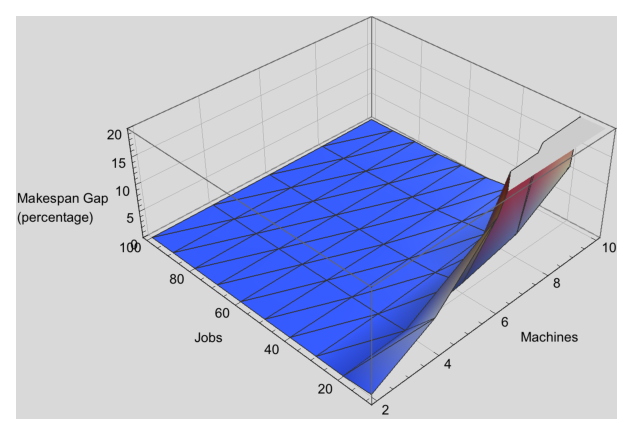
\includegraphics[width=.95\linewidth,height=.7\linewidth]{plots/Q2cRandomMakespanGap.eps}};
  \caption{Random}
  \label{fig:Q1dSFig1}
  \vspace{1cm}
\end{subfigure}%
\begin{subfigure}{.5\textwidth}
  \centering
  \tikz[remember picture]\node[inner sep=0pt,outer sep=0pt] (rates2){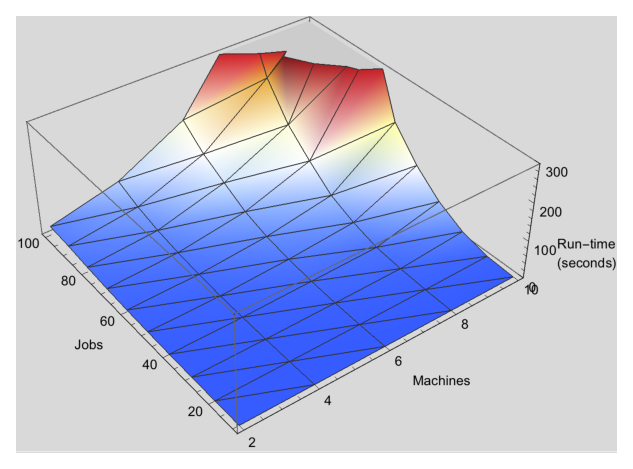
\includegraphics[width=.95\linewidth,height=.7\linewidth]{plots/Q2cRandomRunTime.eps}};
    \caption{Random}
    \label{fig:Q1dSFig2}
    \vspace{1cm}
\end{subfigure}
\begin{subfigure}{.5\textwidth}
  \centering
 \tikz[remember picture]\node[inner sep=0pt,outer sep=0pt] (rates3){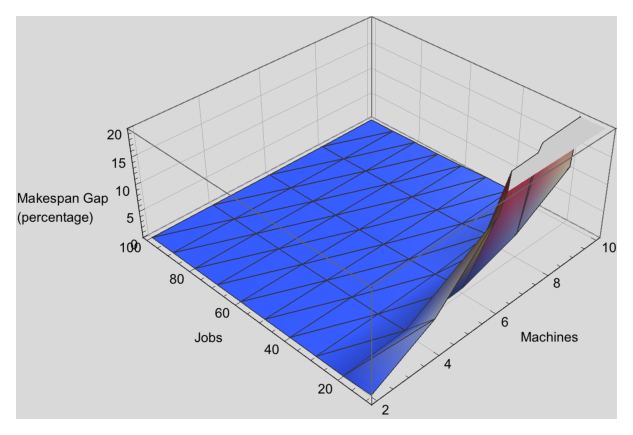
\includegraphics[width=.95\linewidth,height=.7\linewidth]{plots/Q2cGMSMakespanGap.eps}};
   \caption{GMS}
  \label{fig:Q1dSFig3}
\end{subfigure}
\begin{subfigure}{.5\textwidth}
  \centering
  \tikz[remember picture]\node[inner sep=0pt,outer sep=0pt] (rates4){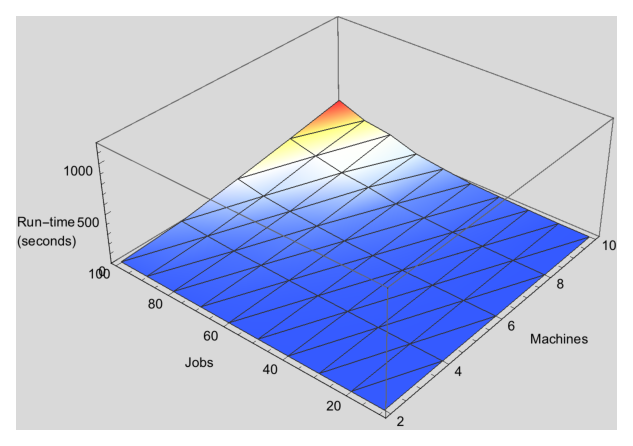
\includegraphics[width=.95\linewidth,height=.7\linewidth]{plots/Q2cGMSRunTime.eps}};
  \caption{GMS}
  \label{fig:Q1dSFig4}
\end{subfigure}
\caption[Experiments VDSS: Random and GMS]{\textbf{Experiments VDS: k=2, using random and GMS initial solution.} \small (a) and (b) display the makespan gap (in percentage) and the run time (in seconds), using a random initial solution. (c) and (d) show the makespan gap (in percentage) and the run time (in seconds), using the GMS initial solution. We only plot makespan gap values between 0 and 20 \%, and run time values between 0 and 1200 s. }
\label{fig:Q2c}

\end{figure}


\newpage
\section{Simulated Annealing Algorithm for MS}
\label{sec:simulatedannealing}

The heuristic we choose to implement is simulated annealing, for which we present detailed pseudo-code in Section \ref{subsec:SA_pseudo}. This algorithm has several free parameters, namely, the neighbourhood function, the cooling schedule which determines the rate at which the temperature decreases, and the initial value of the temperature. We use the same neighbourhood as defined in Section \ref{sec:GLS}. \\

In Section \ref{subsec:initTemp}, we consider an algorithm developed by \citet{ameur2004} to find a good initial value of the temperature. Several cooling schedules are considered, and the results of experiments performed on each are presented in Section \ref{subsec:tempReduc}. Section \ref{subsec:SimAnn_Comp} contains the results of comparing the performance of the simulated annealing heuristic to the performance of the GLS and VDS algorithms. This then motivates Section \ref{subsec:SimAnn_Limit}, in which we push our heuristic to its limits to find the largest possible input instances which can be handled. Finally, in Section \ref{subsec:SolQual}, we conclude by providing other possible methods of determining the quality of a solution and how our heuristic performs with respect to each one.

\subsection{Simulated Annealing Algorithm Pseudocode}
\label{subsec:SA_pseudo}
In our algorithm, we make a slight modification to keep track of the best solution found by the algorithm (Step (3)). In the final step, the best solution is compared to the final solution found by the simulated annealing algorithm. We do this in order to avoid the algorithm returning a worse solution than one previously found. \\

We again use the random or GMS initial feasible solutions, described in Section \ref{sec:implementation}. \\

\emph{Input}: An input instance $I = (p_1,p_2,...,p_n,m)$ of the Makespan Scheduling problem.
\begin{enumerate}
\item Generate an initial feasible solution $\xi = \{\xi_1,\xi_2,...,\xi_n\}$, using Random or GMS. \\
% $T$ = getInitialTemp($I, k, \chi_0, S, p, \epsilon$)
$T := T_0 := 1.5 \times \max\{ \> p_i \>  | i = 1,...,n \}$ (See below for a discussion)
\item $I := 0$ \\
$best:=\xi$
\item\textbf{while} $T>0$ \textbf{do}
\begin{enumerate}
\item Randomly select a neighbour $\beta\in Neigh_x(\alpha)$
\item \textbf{if} makespan($\beta$) $\leq$ makespan($\alpha$) \textbf{then}
\begin{enumerate}
\item $\alpha:=\beta$
\end{enumerate}
\item[] \textbf{else}
\begin{enumerate}
\item Generate a random number $r$ uniformly in the range $(0,1)$
\item \textbf{if} $r<e^{-\frac{\text{makespan}(\alpha)-\text{makespan}(\beta)}{T}}$ \textbf{then}
\begin{enumerate}
\item[] $\alpha:=\beta$
\end{enumerate}
\end{enumerate}
\item \textbf{if}
$\text{makespan}(\alpha) < \text{makespan}(best)$ \textbf{then}
\begin{enumerate}
\item[] $best:=\alpha$
\end{enumerate}
\item $I:=I+1$
\item $T:=\text{reduceTemperature}(T_0,I)$
\end{enumerate}
\item[] \textbf{end while}
\item \textbf{if} $\text{makespan}(\alpha) < \text{makespan}(best)$ \\
\indent \textbf{output}$(\alpha)$ \\
\textbf{else} \\
\indent \textbf{output}$(best)$
\end{enumerate}

\subsection{Choice of the Initial Temperature}
\label{subsec:initTemp}
The performance of the algorithm can vary greatly depending on the initial value of the temperature. We follow the work of Ben-Ameur \citep{ameur2004}, who developed an algorithm to pre-determine the initial temperature $T_0$. \\

In the simulated annealing algorithm presented above, the probability of accepting a bad move (with cost increase) from solution $\alpha$ to $\beta$ is
\begin{equation}
e^{-\frac{\textnormal{cost}(\alpha)-\textnormal{cost}(\beta)}{T}} = e^{-\frac{\textnormal{makespan}(\alpha)-\text{makespan}(\beta)}{T}},
\end{equation}
where $T$ is the current temperature, and $\textnormal{cost}(\alpha) > \textnormal{cost}(\beta)$.
We consider the average probability of accepting a bad move as
\begin{equation}
\pi_\alpha = \frac{e^{-\frac{\text{cost}(\alpha)-\text{cost}(\beta)}{T}}}{\sum_j  \> e^{-\frac{\text{cost}(\alpha)-\text{cost}(\beta_j)}{T}}},
\end{equation}
where we sum over all possible neighbours $\beta_j$ of $\alpha$ (and assume the generation probability of reaching a neighbour is symmetrical, see \citet{ameur2004}). The idea of \citet{ameur2004} is to choose the initial temperature such that the acceptance probability is close to a certain value $\chi_0$ by estimating this acceptance probability based on a random set of neighbours of $\alpha$ which increase the cost. For a full discussion of the algorithm, please refer to \citet{ameur2004}. The pseudo-code of our implementation is described below: \\

\subsubsection*{Algorithm \ref{alg:initTemp}: Initial Temperature Generation}
\label{alg:initTemp}
\emph{Input:}
\begin{itemize}
  \item The input instance $I=(p_1,...,p_n,m)$
  \item $k=2$ exchange value
  \item The desired acceptance probability $\chi_0 = 0.8$
  \item The number of random transitions to generate $S = 1000$
  \item A stopping criterion $\epsilon = 0.001$
\end{itemize}
\begin{enumerate}
  \item Generate a set, $\mathcal{S}$, of size $S$, of random transitions:
  \item[] For each random transition, we generate a random initial solution $\alpha$ and move to a random neighbour $\beta$. We let $E_\textnormal{max} := \min\{\textnormal{cost}(\alpha),\textnormal{cost}(\beta)\}$ and $E_{\textnormal{min}} := \max\{\textnormal{cost}(\alpha),\textnormal{cost}(\beta)\}$ for each transition $S$.
  \item $T_1:= - \frac{\sum_{t \in S} E_{\textnormal{max}_t} - E_{\textnormal{min}_t}}{|S| \textnormal{ln}(\xi_0)}$
  \item[] Let $n=1$
  \item[] Compute $\chi(T):=\frac{\displaystyle\sum\limits_{t\in \mathcal{S}} e^\frac{E_{{max}_{t}}}{T_n}}{\displaystyle\sum\limits_{t\in \mathcal{S}} e^\frac{E_{{min}_{t}}}{T_n}}$
  \item \textbf{while} $|\chi(T_n)-\chi_0|>\epsilon$ \textbf{do}
  \begin{enumerate}
    \item $T_{n+1} := T_{n} \cdot(\frac{\ln(\chi(T_n))}{\ln(\chi_0)})^{\frac{1}{p}}$
    \item Compute $\chi(T_n)$
  \end{enumerate}
  \item \textbf{output} $T_n$
\end{enumerate}

We will use this algorithm to generate the initial temperature for test cases with $n=$ 10, 20, 30, 40, 50, 60, 70, 80, 90, 100 and $m=$ 2, 4, 6, 8, 10, in order to get an idea of how large the initial temperature should be for these instances. We do this 100 times per combination of $n$ and $m$, with processing times uniformly distributed between 1 and 100, and calculate the average. The averaged results are shown in Table \ref{tab:Q3InitialTemp} and Figure \ref{fig:Initialtemperature}. We see that the initial temperature is larger when the number of machines is small, and the number of jobs is large. There is more variation in the initial temperature varying the number of machines than the number of jobs. By performing a few more test instances with smaller and larger processing times (with self-made instances and not shown in this report), we found that choosing an initial temperature of approximately 1.5 times larger than the largest processing time in an instance gives good results (and is faster, since we do not need to call the algorithm by \citet{ameur2004} for every run of our simulated annealing algorithm). We can also see that this approximately holds for the instances in Figure \ref{fig:Initialtemperature}, since the processing times are uniformly distributed between 1 and 100, and the temperature is approximately 150 for a small number of machines.


\begin{figure}[H]
\begin{center}
{\large \bf  Initial Temperature for Simulated Annealing}
\end{center}
\begin{subfigure}{\textwidth}
  \centering
  \tikz[remember picture]\node[inner sep=0pt,outer sep=0pt] (rates1){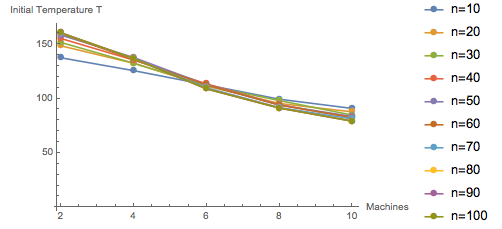
\includegraphics[width=.7\linewidth,height=.4\linewidth]{plots/InitialTemperature.png}};
\end{subfigure}%
\caption{The initial temperatures generated by the algorithm by \citet{ameur2004}, using 100 realisations per $n$ and $m$, processing times between 1 and 100, and the random initial solution.}
\label{fig:Initialtemperature}
\end{figure}




\subsection{Choice of the Temperature Reduction Function: \emph{reduceTemperature}}
\label{subsec:tempReduc}

We consider several options for the cooling schedule, which is called \textit{reduceTemperature}$(T_0,I)$ in the pseudocode of Section \ref{subsec:SA_pseudo}. All are functions, $f$, of the initial temperature, $T_0$, and the iteration number, $I$. \\

\textbf{Exponential multiplicative cooling}
\begin{flalign*}
& f_1(T_0,I)=T_0\cdot \mu^I & \\
& \text{where we set } \mu=0.8. &
\end{flalign*}

\textbf{Simple exponential cooling}
\begin{flalign*}
f_2(T_0,I)=T_0 - I &&
\end{flalign*}

\textbf{Linear multiplicative cooling}
\begin{flalign*}
f_3(T_0,I)=\frac{1}{1+I}\cdot T_0 &&
\end{flalign*}

\textbf{Quadratic multiplicative cooling}
\begin{flalign*}
f_4(T_0,I)=\frac{1}{1+I^2}\cdot T_0 &&
\end{flalign*}

We experiment with the four possible cooling functions to use for the simulated annealing algorithm: simple linear cooling, linear multiplicative cooling, quadratic multiplicative cooling and exponential multiplicative cooling. We implemented the simulated annealing algorithm of Section \ref{subsec:SA_pseudo} in Python. See \emph{ourHeuristic} in MS\_heuristics.py. \\

For $n=10,20,30,40,50,60,70,80,90,100$ and $m=2,4,6,8,10$, we run our simulated annealing algorithm 10 times, using a random initial solution. The averaged results are given in Table \ref{tab:Q3Cooling} and \ref{tab:Q3CoolingQuadMult}, and in Figure \ref{fig:Q3CoolingFig1} and \ref{fig:Q3CoolingFig2}. \\

We find that the quadratic multiplicative function to be by far the slowest, taking between ten and a hundred times as long as the other methods. However, the makespan gap is always lower, and more than 10 times lower when $n>50$ and $m>6$ for the quadratic multiplicative method. We see that when the number of jobs is close to the number of machines, the makespan gaps are comparable for all methods. Because the quadratic multiplicative method has a better solution quality, we choose to continue with this cooling schedule. \\

In the next section, we investigate the best choice of initial solution to use.

\begin{figure}[H]
\begin{center}
{\Large \bf Simulated Annealing Cooling Function Experiments}
\end{center}
\begin{subfigure}{.5\textwidth}
  \centering
  \tikz[remember picture]\node[inner sep=0pt,outer sep=0pt] (rates1){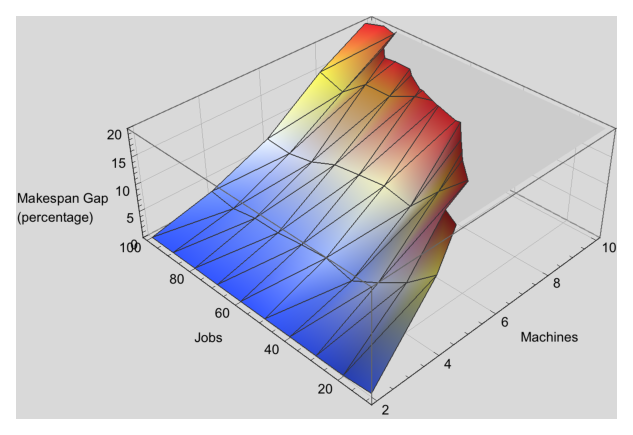
\includegraphics[width=.95\linewidth,height=.7\linewidth]{plots/Q3CoolingSimpleMakespanGap.eps}};
  \caption{Simple Linear Makespan Gap}
  \label{fig:Q3CoolingSFig1}
  \vspace{1cm}
\end{subfigure}%
\begin{subfigure}{.5\textwidth}
  \centering
  \tikz[remember picture]\node[inner sep=0pt,outer sep=0pt] (rates2){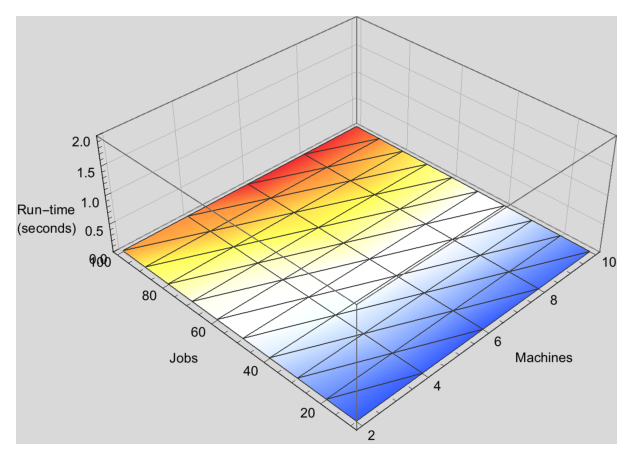
\includegraphics[width=.95\linewidth,height=.7\linewidth]{plots/Q3CoolingSimpleRuntime.eps}};
    \caption{Simple Linear Run time}
    \label{fig:Q3CoolingSFig2}
    \vspace{1cm}
\end{subfigure}
\begin{subfigure}{.5\textwidth}
  \centering
 \tikz[remember picture]\node[inner sep=0pt,outer sep=0pt] (rates3){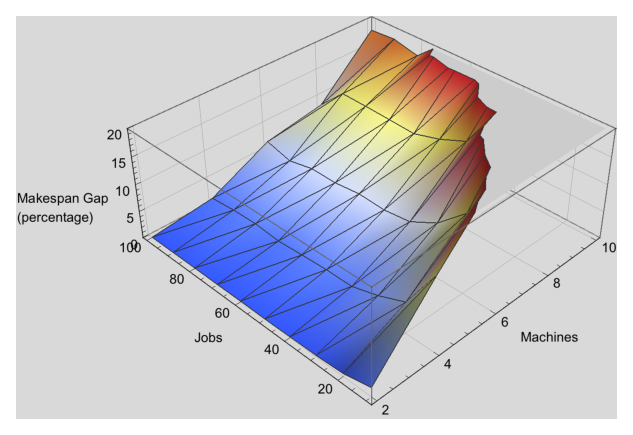
\includegraphics[width=.95\linewidth,height=.7\linewidth]{plots/Q3CoolingLinMultMakespanGap.eps}};
   \caption{Linear Multiplicative Makespan Gap}
  \label{fig:Q3CoolingSFig3}
\end{subfigure}
\begin{subfigure}{.5\textwidth}
  \centering
  \tikz[remember picture]\node[inner sep=0pt,outer sep=0pt] (rates4){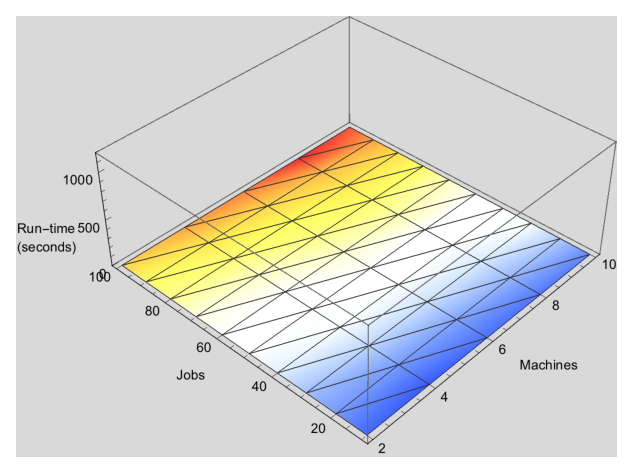
\includegraphics[width=.95\linewidth,height=.7\linewidth]{plots/Q3CoolingLinMultRuntime.eps}};
  \caption{Linear Multiplicative Run time}
  \label{fig:Q3CoolingSFig4}
\end{subfigure}
\caption[Experiments Simulated Annealing: Cooling Schedules]{\textbf{Experiments Simulated Annealing: simple linear and linear multiplcative cooling functions.} \small (a) and (b) display the makespan gap (in percentage) and the run time (in seconds), using a simple linear cooling function. (c) and (d) show the makespan gap (in percentage) and the run time (in seconds), using a linear multiplicative cooling function. We only plot makespan gap values between 0 and 20 \%, and run time values between 0 and 1200 s. }
\label{fig:Q3CoolingFig1}

\end{figure}

\begin{figure}[H]
\begin{center}
{\Large \bf Simulated Annealing Cooling Function Experiments}
\end{center}
\begin{subfigure}{.5\textwidth}
  \centering
  \tikz[remember picture]\node[inner sep=0pt,outer sep=0pt] (rates1){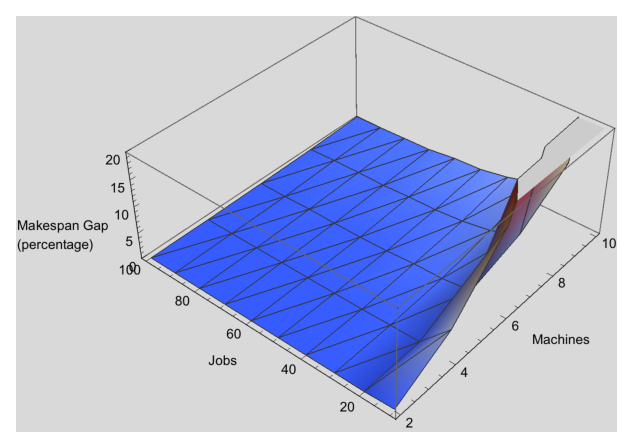
\includegraphics[width=.95\linewidth,height=.7\linewidth]{plots/Q3CoolingQuadMultMakespanGap.eps}};
  \caption{Quadratic Multiplicative Makespan Gap}
  \label{fig:Q3CoolingSFig5}
  \vspace{1cm}
\end{subfigure}%
\begin{subfigure}{.5\textwidth}
  \centering
  \tikz[remember picture]\node[inner sep=0pt,outer sep=0pt] (rates2){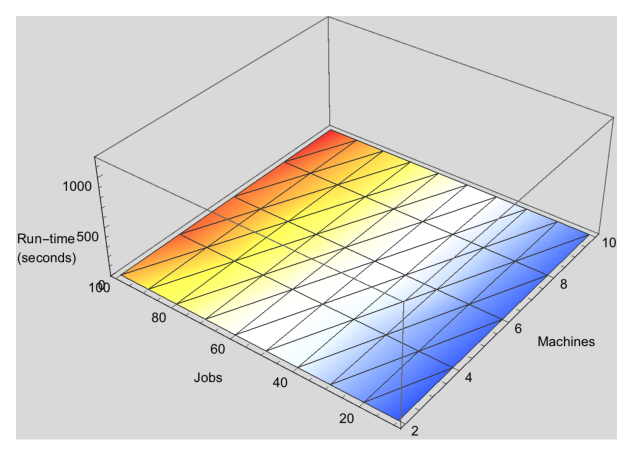
\includegraphics[width=.95\linewidth,height=.7\linewidth]{plots/Q3CoolingQuadMultRuntime.eps}};
    \caption{Quadratic Multiplicative Runtime}
    \label{fig:Q3CoolingSFig6}
    \vspace{1cm}
\end{subfigure}
\begin{subfigure}{.5\textwidth}
  \centering
 \tikz[remember picture]\node[inner sep=0pt,outer sep=0pt] (rates3){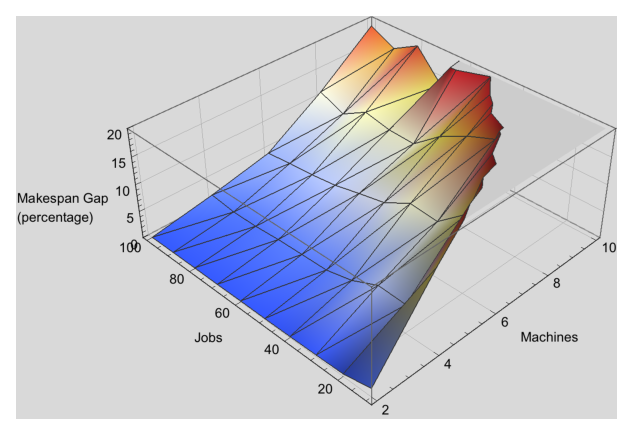
\includegraphics[width=.95\linewidth,height=.7\linewidth]{plots/Q3CoolingExpMultMakespanGap.eps}};
   \caption{Exponential Multiplicative Makespan Gap}
  \label{fig:Q3CoolingSFig7}
\end{subfigure}
\begin{subfigure}{.5\textwidth}
  \centering
  \tikz[remember picture]\node[inner sep=0pt,outer sep=0pt] (rates4){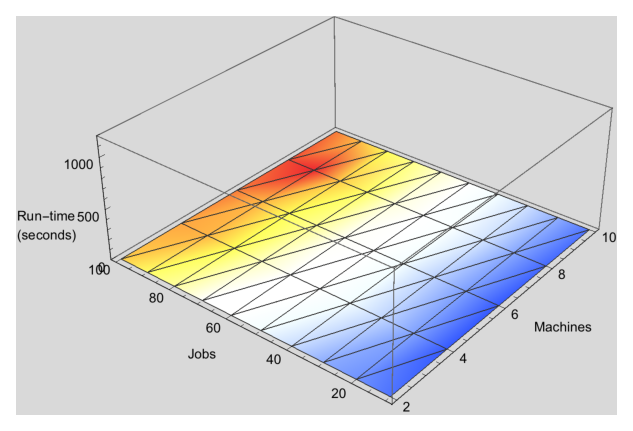
\includegraphics[width=.95\linewidth,height=.7\linewidth]{plots/Q3CoolingExpMultRuntime.eps}};
  \caption{Exponential Multiplicative Runtime}
  \label{fig:Q3CoolingSFig8}
\end{subfigure}
\caption[Experiments Simulated Annealing: Cooling Schedules]{\textbf{Experiments Simulated Annealing: quadratic and exponential multiplicative cooling functions.} \small (a) and (b) display the makespan gap (in percentage) and the run time (in seconds), using a quadratic multiplicative cooling function. (c) and (d) show the makespan gap (in percentage) and the run time (in seconds), using a exponential multiplicative cooling function. We only plot makespan gap values between 0 and 20 \%, and run time values between 0 and 1200 s. }
\label{fig:Q3CoolingFig2}

\end{figure}



\subsection*{Choice of Initial Solution}
We test both random and GMS initial solutions for our heuristic procedure. The results of 10 realisations per $n$ and $m$ are shown in Table \ref{tab:Q3SimulatedAnnealing} and Figure \ref{fig:Q3InitSol}. We see that the random and GMS initial solution give similar results. The average makespan gap over all $n$ and $m$ for the random initial solution is 3.69 \%, while for the GMS initial solution it is 3.55 \%. The average run time over all $n$ and $m$ for the random initial solution is 1.19 s, while for the GMS initial solution it is 1.22 s. Hence, like GLS and VDS, the performance of our simulated annealing algorithm is not affected by a choice between these two initial solution methods.


\begin{figure}[H]
\begin{center}
{\Large \bf Simulated Annealing Initial Solution Experiments}
\end{center}
\begin{subfigure}{.5\textwidth}
  \centering
  \tikz[remember picture]\node[inner sep=0pt,outer sep=0pt] (rates1){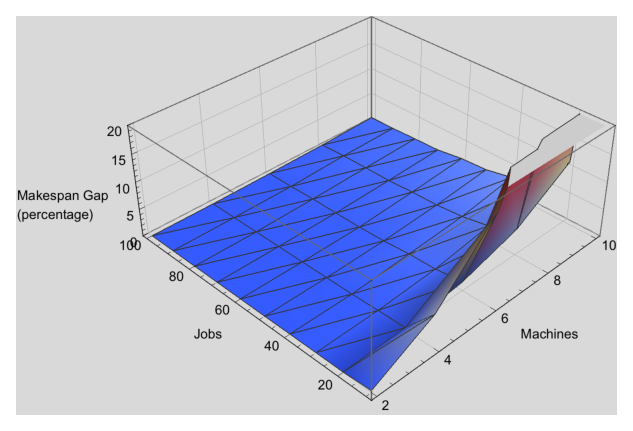
\includegraphics[width=.95\linewidth,height=.7\linewidth]{plots/Q3RandomMakespanGap.eps}};
  \caption{Random}
  \label{fig:Q3InitSolSFig1}
  \vspace{1cm}
\end{subfigure}%
\begin{subfigure}{.5\textwidth}
  \centering
  \tikz[remember picture]\node[inner sep=0pt,outer sep=0pt] (rates2){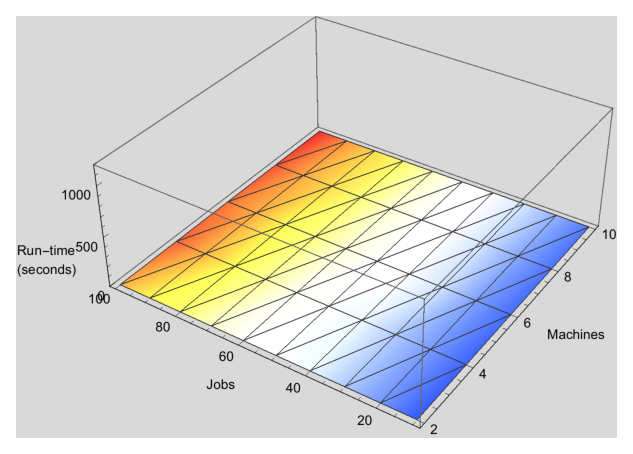
\includegraphics[width=.95\linewidth,height=.7\linewidth]{plots/Q3RandomRunTime.eps}};
    \caption{Random}
    \label{fig:Q3InitSolSFig2}
    \vspace{1cm}
\end{subfigure}
\begin{subfigure}{.5\textwidth}
  \centering
 \tikz[remember picture]\node[inner sep=0pt,outer sep=0pt] (rates3){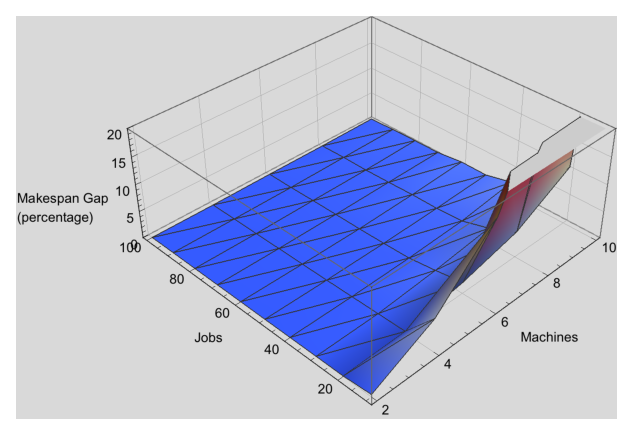
\includegraphics[width=.95\linewidth,height=.7\linewidth]{plots/Q3GMSMakespanGap.eps}};
   \caption{GMS}
  \label{fig:Q3InitSolSFig3}
\end{subfigure}
\begin{subfigure}{.5\textwidth}
  \centering
  \tikz[remember picture]\node[inner sep=0pt,outer sep=0pt] (rates4){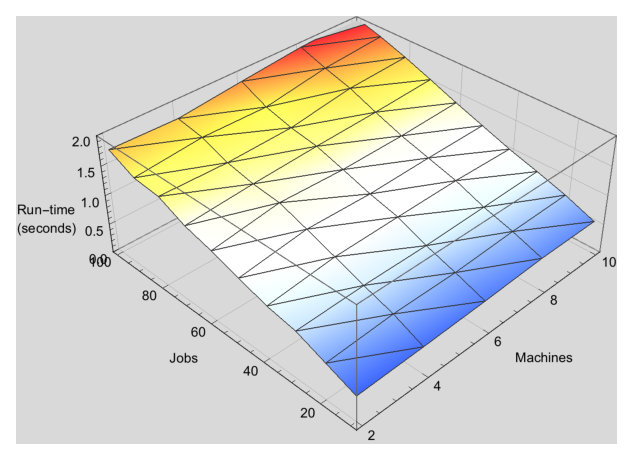
\includegraphics[width=.95\linewidth,height=.7\linewidth]{plots/Q3GMSRunTime.eps}};
  \caption{GMS}
  \label{fig:Q3InitSolSFig4}
\end{subfigure}
\caption[Experiments Simulated Annealing: Initial Solution]{\textbf{Experiments Simulated Annealing: random and GMS initial solutions.} \small (a) and (b) display the makespan gap (in percentage) and the run time (in seconds), using a random initial solution. (c) and (d) show the makespan gap (in percentage) and the run time (in seconds), using the GMS initial solution. We only plot makespan gap values between 0 and 20 \%, and run time values between 0 and 1200 s. }
\label{fig:Q3InitSol}

\end{figure}

\subsection{Comparison to GLS and VDS} \label{subsec:SimAnn_Comp}
We can compare the makespan gaps and run times of our simulated annealing solutions with GLS and VDS. 
Comparing tables \ref{tab:Q1d}, \ref{tab:Q2d}, and \ref{tab:Q3SimulatedAnnealing}, and their respective figures \ref{fig:Q1d}, \ref{fig:Q2c}, and \ref{fig:Q3InitSol}, we see that the makespan gaps by the simulated annealing algorithm are comparable to the makespan gaps by VDS. However, the run time of the simulated annealing algorithm is much faster, with average run time over all $n$ and $m$ (1.19 s for the random initial solution and 1.22 s for the GMS initial solution) much faster than the average run time of VDS (79.30 s for the random initial solution and 42.69 s for the GMS initial solution), and more than 100 times faster than GLS (176.74 s for the random initial solution and 171.04 s for the GMS initial solution). \\

In addition, in Table \ref{tab:Q2d} and \ref{tab:Q3SimulatedAnnealing}, we see that the makespan gap when $n$ and $m$ are comparable (or equal when $n=m=10$) is approximately equal for VDS and simulated annealing. As noted in Section \ref{sec:selectingk}, our measure of solution quality (makespan gap) is bad in these cases. However, we can see that VDS and simulated annealing have similar results for these cases. In Section \ref{subsec:SolQual}, we will address this issue and compare the results of our simulated annealing algorithm to solutions given by an exact algorithm (MIP). 

\subsection{Performance Limitations} \label{subsec:SimAnn_Limit}
To test the performance limitations of the simulated annealing algorithm we experiment with very large input instances. By choosing to use the slowest of the cooling functions (i.e. quadratic multiplicative cooling) we may have limited the size of input instances that our algorithm could handle in a reasonable amount of time. Even so, instances with 10,000 jobs still terminate within 10 minutes. \\

So far the input instances we generated had a uniform distribution of processing times between 1 and some constant maximum value. We chose the maximum processing time to be 100 for all the instances we generated for testing the limitations of the GLS and VDS algorithms. However, the processing times of the jobs and their distribution could also influence the solution quality. \\

In order to demonstrate this, we let the maximum processing time be defined as a function of $n$, namely: $\text{max-processing-time}=n/10$. The division by 10 here is an artefact of our heuristic being implemented in Python, as when we tested the input instance of 1,000,000 jobs and 2 machines, calculating the total load of a machine required storing scalar values. Without the assistance of 3rd party packages, Python cannot store scalar values larger than $2^{31}$ and so this calculation resulted in overflow errors. Dividing by 10 solved this issue for the size of the instances we aimed to test. \\

For these experiments we vary the number of jobs but kept the number of machines constant at $m=2$. Our initial testing indicated that when $n$ became 2 orders of magnitude larger than $m$, the exact number of machines began to have very little influence on the results. Note, in Table \ref{tab:Q3SimulatedAnnealingruntimeRandom} and  \ref{tab:Q3SimulatedAnnealingruntimeGMS} and Figure \ref{fig:Q3InitSol}, the run time does not vary much with $m$. So, instead of testing $n=$ 100, 500, 1000, 5,000, 10,000 and 50,000 against a range of $m$ values, we chose $m$ to be a constant, thus saving computation time and still achieving the desired outcome of testing simulated annealing's limits. \\

\subsubsection{Engineering Poor Input Instances}
We aim to create instances of the problem which are particularly difficult to solve to optimality. To this end, we investigate ways to distribute the processing times between 1 and $n/10$ other than simply using the uniform distribution. \\

{\bf Poor Distribution Definition} \\
In order to create these instances, we first generate a new probability distribution function for the processing times. This distribution function makes it more likely to select either very small or very large processing times for the jobs. Specifically, we give processing times in the lowest 5 \% and highest 5 \% of a pre-specified maximum processing time the highest probability, in such a way that the total probability of jobs having processing time within 5 \% of 0 or the maximum is 0.9. With this probability density function, we then select processing times using Python's (Numpy) random inbuilt random number generator, which takes the probability density function as input. \\

We consider instances where the processing times are almost exclusively concentrated near the minimum and maximum possible values. We are motivated to try such a distribution as the makespan values between most neighbouring solutions will have a high level of volatility. Given $k=2$ and a jump-neighbourhood, this is demonstrated as follows; consider any two jobs which in iteration $i$ of the simulated annealing algorithm are chosen to be exchanged. Given the distribution we construct heavily weights the concentration of processing times to very large and very small values, we can assume almost certainly that the processing times of these jobs will be near 1 or $\frac{n}{10}$. The neighbourhood of our current solution will contain a large amount of exchanges that have little if any affect on the makespan (when moving small jobs), together with a large amount of neighbours which will have wildly large affects (when moving large jobs). \\

An instance with such a poor distribution of processing times will have a volatile neighbourhood topology. This should result in simulated annealing having more difficulty in finding the good local optima.

\subsubsection{Results of Performance Limits Experiments}
The averaged results of 10 realisations for large $n$ and $m=2$ are shown in Tables \ref{tab:Q3Limitsresults} and Figure \ref{fig:Q3Limit}, for both the uniform and the poor distributions of processing times between 0 and $n/10$. We see that the makespan gap decreases with approximate slope 1, as $n$ increases. This gives that the makespan gap is of $O(1/n)$. The run time increases as $n$ increases and is approximately of $O(n^2)$. \\

We also find that when the instance size became exceedingly large, using a uniform distribution of processing times (in blue) made the simulated annealing algorithm find close to optimal solutions more easily than the new distribution (in red). This indicates that our poor distribution of processing times is slightly more difficult for simulated annealing to solve. Moreover, as $n$ and $m$ increase we can conclude that the large and small processing times in our pathological distribution `even out' and make the problem easier to solve.



\begin{figure}[H]
\begin{center}
{\Large \bf Simulated Annealing Performance Experiments}
\end{center}
\begin{subfigure}{.5\textwidth}
  \centering
  \tikz[remember picture]\node[inner sep=0pt,outer sep=0pt] (rates1){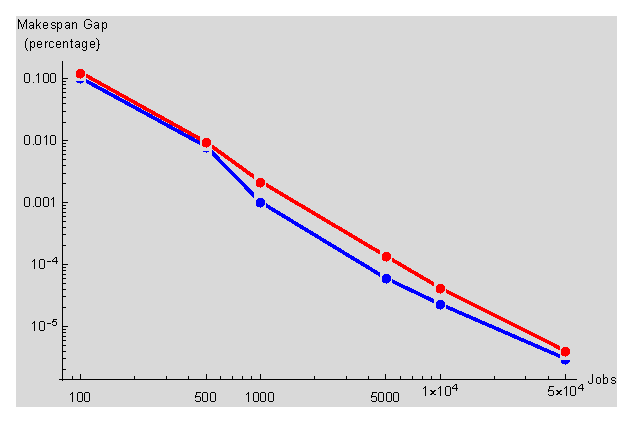
\includegraphics[width=.95\linewidth,height=.7\linewidth]{plots/Q3LimitMakespanGap.eps}};
  \caption{Makespan Gap}
  \label{fig:Q3LimitSFig1}
\end{subfigure}%
\begin{subfigure}{.5\textwidth}
  \centering
  \tikz[remember picture]\node[inner sep=0pt,outer sep=0pt] (rates2){\includegraphics[width=.95\linewidth,height=.7\linewidth]{plots/Q3LimitRuntime.eps}};
    \caption{Run time}
    \label{fig:Q3LimitSFig2}
\end{subfigure}
\caption[Experiments Simulated Annealing: Limits]{\textbf{Experiments Simulated Annealing.} \small Blue line: uniform distribution, red line: pathological distribution. (a) and (b) display the makespan gap (in percentage) and the run time (in seconds), using both types of distributions. We only plot makespan gap values between 0 and 20 \%, and run time values between 0 and 1200 s. The results are also given in Table \ref{tab:Q3Limitsresults}.}
\label{fig:Q3Limit}

\end{figure}

\newpage
\subsection{Methods of Determining Solution Quality} \label{subsec:SolQual}
So far, we have measured the solution quality by calculating the makespan gap, as explained in Section~\ref{sec:implementation}, Equation (\ref{eq:NaiveMakespanGap}). We saw that when $n$ is close to $m$, the makespan gap is quite large, and also when $n=m=10$ although the solution is optimal. The lower bound we calculated with Equation (\ref{eq:NaiveLB}), assuming the processing times of the jobs are fractional, is too low because it is less likely that each machine has a similar total processing time.  \\

\subsubsection{Other measures of solution quality}
\color{red}
Another possible strategy for measuring the solution quality is to calculate the ratio between of the makespan output by GMS, described in Section \ref{sec:implementation}, and the makespan output of our simulated annealing algorithm. When we take the GMS as initial solution in the simulated annealing algorithm, the final makespan of our heuristic can not be worse than GMS, since we save the current best solution and output this if no better solution is found. We re-run the simulated annealing algorithm for the instances of MS we saved and used for GLS and VDS in Table \ref{tab:Q1d} and \ref{tab:Q2d}, and also determine the optimal solution using ....
GMS is an 4/3-approximation algorithm.... 
\color{black}


\subsubsection{Constraint Programming}
We can calculate whether our solution is optimal by taking the ratio between the solution output by our simulated annealing algorithm and the optimal solution.



\todo[inline]{Detail on true implementation of MP, in bash?}


\todo[inline]{*insert table with 100\% in all entries here*}


\section{Conclusion}
We conclude that our simulated annealing algorithm is much faster than GLS and VDS for the MS input instances we have seen, while producing solutions of similar quality as VDS. We initially measured the quality of GLS, VDS, and our heuristic using the makespan gap, which uses the lower bound of the total processing time assuming all processing times are fractional.......... 


\newpage
\bibliography{references}{}
\bibliographystyle{apalike}

\newpage

\section{Appendix}
\subsection*{Full results for GLS experiments}
\begin{table}[H]
\begin{center}
{\large \bf GLS Experiments with Random Initial Solution}
\end{center}
\begin{center}
{\large \bf $k=1$}
\end{center}
\centering
\begin{subtable}{0.48\textwidth}
\centering
\caption[Makespan gap]{Makespan gap}
%\renewcommand\arraystretch{1.3}
\renewcommand\tabcolsep{1pt}
\centering
\footnotesize
\begin{tabular}{l|*{9}{c}}
\backslashbox{m}{n} & 15 & 20 & 25 & 30 & 35 & 40 & 45 & 50 \\
\hline
2 & 1.40 & 0.35 & 0.34 & 0.15 & 0.14 & 0.09 & 0.04 & 0.07  \\
4 & 5.93 & 2.84 & 2.51 & 1.43 & 1.56 & 0.84 & 0.88 & 0.69 \\
6 & 11.99 & 10.06 & 5.62 & 3.73 & 2.74 & 3.00 & 2.58 & 1.93 \\
8 & 17.85 & 12.18 & 13.44 & 12.42 & 8.11 & 6.45 & 5.03 & 3.81 \\
10 & 40.01 & 19.70 & 14.06 & 18.40 & 14.12 & 9.98 & 12.30 & 10.50  \\
\end{tabular}
\label{tab:Q1ck=1makespangap}
\end{subtable}
\begin{subtable}{0.48\textwidth}
\centering
\caption[Run time]{Run time}
%\renewcommand\arraystretch{1.3}
\renewcommand\tabcolsep{1pt}
\centering
\footnotesize
\begin{tabular}{l|*{9}{c}}
\backslashbox{m}{n} & 15 & 20 & 25 & 30 & 35 & 40 & 45 & 50 \\
\hline
2& 0.001& 0.002&  0.003&  0.003&  0.005&  0.005&  0.008&  0.009 \\
4& 0.004& 0.008&  0.011&  0.018&  0.024&  0.032&  0.045&  0.044 \\
6& 0.013& 0.019&  0.030&  0.043&  0.058&  0.067&  0.093&  0.096 \\
8& 0.020& 0.036&  0.043&  0.075&  0.102&  0.150&  0.217&  0.219 \\
10& 0.026& 0.060&  0.081&  0.135&  0.179&  0.200&  0.325&  0.385
\end{tabular}
\label{tab:Q1ck=1runtime}
\end{subtable}
\begin{center}
\vspace{0.6cm}
{\large \bf $k=2$}
\end{center}
\begin{subtable}{0.48\textwidth}
\centering
\caption[Makespan gap]{Makespan gap}
%\renewcommand\arraystretch{1.3}
\renewcommand\tabcolsep{1pt}
\centering
\footnotesize
\begin{tabular}{l|*{9}{c}}
\backslashbox{m}{n} & 15 & 20 & 25 & 30 & 35 & 40 & 45 & 50 \\
\hline
2& 0.14&  0&  0.08& 0.06& 0&  0.05& 0.04& 0.04 \\
4& 0.12&  0.22& 0.21& 0.06& 0.17& 0.09& 0.04& 0 \\
6& 4.87&  1.11& 2.59& 1.49& 0.53& 0.37& 0.24& 0.30 \\
8& 32.00& 7.36& 0.85& 0.95& 0.78& 0.76& 0.42& 0.76 \\
10 &65.48&  7.61& 8.24& 3.38& 2.89& 1.53& 0.56& 0.83
\end{tabular}
\label{tab:Q1ck=2makespangap}
\end{subtable}
\begin{subtable}{0.48\textwidth}
\centering
\caption[Run time]{Run time}
%\renewcommand\arraystretch{1.3}
\renewcommand\tabcolsep{1pt}
\centering
\footnotesize
\begin{tabular}{l|*{9}{c}}
\backslashbox{m}{n} & 15 & 20 & 25 & 30 & 35 & 40 & 45 & 50 \\
\hline
2& 0.02&  0.05& 0.05& 0.07& 0.11& 0.45& 0.72& 1.09 \\
4& 0.18&  0.78& 0.64& 0.73& 2.40& 4.68& 7.40& 5.21 \\
6& 0.50&  0.87& 3.27& 2.82& 8.53& 19.86&  11.44&  29.11 \\
8& 1.02&  3.38& 8.65& 17.52&  21.71&  42.08&  49.94&  94.56 \\
10& 2.30& 5.59& 10.94&  23.56&  59.58&  53.83&  100.87& 195.12 \\
\end{tabular}
\label{tab:Q1ck=2runtime}
\end{subtable}
\begin{center}
\vspace{0.6cm}
{\large \bf $k=3$}
\end{center}
\begin{subtable}{0.48\textwidth}
\centering
\caption[Makespan gap]{Makespan gap}
%\renewcommand\arraystretch{1.3}
\renewcommand\tabcolsep{1pt}
\centering
\footnotesize
\begin{tabular}{l|*{9}{c}}
\backslashbox{m}{n} & 15 & 20 & 25 & 30 & 35 & 40 & 45 & 50 \\
\hline
2& 0.14&	0.06&	0&	0.02&	0.07&	0.82&	0.09&	0.04 \\
4& 0.20&	0.41&	0.14&	0.12&	0.20&	0.08&	0.08&	0.11 \\
6& 2.45&	1.65&	0.56&	0.12&	0.10&	0.16&	0.08&	0.04 \\
8& 12.88&	4.13&	0.42&	0.37&	0.96&	0.42&	0.40&	0.41 \\
10& 17.59&	2.27&	3.09&	1.10&	0.86&	0.93&	0.40&	0.26
\end{tabular}
\label{tab:Q1ck=3makespangap}
\end{subtable}
\begin{subtable}{0.48\textwidth}
\centering
\caption[Run time]{Run time}
%\renewcommand\arraystretch{1.3}
\renewcommand\tabcolsep{1pt}
\centering
\scriptsize
\begin{tabular}{l|*{9}{c}}
\backslashbox{m}{n} & 15 & 20 & 25 & 30 & 35 & 40 & 45 & 50 \\
\hline
2& 0.09&	0.50&	1.12&	1.72&	4.00&	11.55&	17.01&	28.55 \\[1.5ex]
4& 1.21&	7.75&	14.09&	34.79&	56.88&	121.77&	291.35&	505.66 \\[1.5ex]
6& 7.90&	25.3&	64.16&	131.15&	244.04&	980.48&	1262.60&	2590.84 \\[1.5ex]
8& 19.78&	80.02&	194.86&	435.55&	987.58&	2624.76&	3264.98&	5114.31 \\[1.5ex]
10& 54.73&	153.17&	347.68&	604.12&	2002.52&	4088.55&	6251.35&	15462.72
\end{tabular}
\label{tab:Q1ck=3runtime}
\end{subtable}
\caption{GLS Experiments: $k=1,2,3$, using a random initial solution. The makespan gap is given in \% and the run time in seconds.}
\label{tab:Q1c}
\end{table}



\begin{comment}
\begin{table}
\begin{center}
{\large \bf GLS Experiments with GMS Initial Solution}
\end{center}
\begin{center}
{\large \bf $k=1$}
\end{center}
\centering
\begin{subtable}{0.48\textwidth}
\centering
\caption[Makespan gap]{Makespan gap}
%\renewcommand\arraystretch{1.3}
\renewcommand\tabcolsep{1pt}
\centering
\footnotesize
\begin{tabular}{l|*{9}{c}}
\backslashbox{m}{n} & 15 & 20 & 25 & 30 & 35 & 40 & 45 & 50 \\
\hline
2& 0.87&  0.11& 0.08& 0.39& 0.13& 0&  0.05& 0 \\
4& 4.35&  2.38& 1.48& 0.86& 0.38& 0.22& 0.46& 0 \\
6& 7.71&  4.16& 2.04& 1.60& 0.44& 1.37& 2.15& 1.20 \\
8& 5.50&  7.32& 1.38& 4.85& 1.86& 1.39& 2.95& 0.80 \\
10& 49.55&  7.72& 5.01& 5.23& 6.09& 1.33& 3.50& 2.30
\end{tabular}
\label{tab:Q1ck=1makespangapGMS}
\end{subtable}
\begin{subtable}{0.48\textwidth}
\centering
\caption[Run time]{Run time}
%\renewcommand\arraystretch{1.3}
\renewcommand\tabcolsep{1pt}
\centering
\footnotesize
\begin{tabular}{l|*{9}{c}}
\backslashbox{m}{n} & 15 & 20 & 25 & 30 & 35 & 40 & 45 & 50 \\
\hline
2& 0.0005&  0.001&  0.001&  0.001&  0.002&  0.002&  0.003&  0.003 \\
4& 0.002& 0.003&  0.002&  0.006&  0.008&  0.005&  0.012&  0.007 \\
6& 0.003& 0.002&  0.01& 0.013&  0.006&  0.013&  0.040&  0.018 \\
8& 0.004& 0.012&  0.009&  0.022&  0.014&  0.010&  0.034&  0.066 \\
10& 0.024&  0.012&  0.026&  0.035&  0.045&  0.011&  0.055&  0.098
\end{tabular}
\label{tab:Q1ck=1runtimeGMS}
\end{subtable}
\begin{center}
\vspace{0.6cm}
{\large \bf $k=2$}
\end{center}
\begin{subtable}{0.48\textwidth}
\centering
\caption[Makespan gap]{Makespan gap}
%\renewcommand\arraystretch{1.3}
\renewcommand\tabcolsep{1pt}
\centering
\footnotesize
\begin{tabular}{l|*{9}{c}}
\backslashbox{m}{n} & 15 & 20 & 25 & 30 & 35 & 40 & 45 & 50 \\
\hline
2& 0& 0&  0.09& 0&  0.05& 0.06& 0.05& 0 \\
4& 0.67&  0.43& 0.3&  0&  0.12& 0.05& 0.05& 0.04 \\
6& 2.65&  0.70& 0.89& 0.82& 0.29& 0.25& 0.19& 0.08 \\
8& 13.54& 1.21& 0.53& 0.70& 0.53& 0.35& 0.16& 0.50 \\
10& 7.75& 19.6& 3.10& 2.56& 2.47& 1.07& 0.87& 0.66
\end{tabular}
\label{tab:Q1ck=2makespangapGMS}
\end{subtable}
\begin{subtable}{0.48\textwidth}
\centering
\caption[Run time]{Run time}
%\renewcommand\arraystretch{1.3}
\renewcommand\tabcolsep{1pt}
\centering
\footnotesize
\begin{tabular}{l|*{9}{c}}
\backslashbox{m}{n} & 15 & 20 & 25 & 30 & 35 & 40 & 45 & 50 \\
\hline
2& 0.02&  0.03& 0.05& 0.08& 0.22& 0.68& 0.71& 0.28 \\
4& 0.1& 0.37& 0.46& 0.44& 1.97& 2.49& 4.22& 5.5 \\
6& 0.77&  0.71& 2.1&  6.81& 6.08& 10.06&  17.3& 19.14 \\
8& 1.11&  1.14& 2.76& 11.8& 6.81& 32.03&  33.08&  77.17 \\
10& 1.47& 4.42& 7.41& 18.62&  49.96&  40.49&  54.06&  190.83
\end{tabular}
\label{tab:Q1ck=2runtimeGMS}
\end{subtable}
\begin{center}
\vspace{0.6cm}
{\large \bf $k=3$}
\end{center}

\end{table}
\end{comment}

\newpage
\begin{table}[h]
\begin{center}
{\Large \bf GLS Experiments}
\end{center}
\begin{center}
{\large Random initial solution}
\end{center}
\raggedright
%\caption{k=1 \color{red} AND SAME TABLES FOR K=2 AND K=3, PREFER NEXT TO EACH OTHER \color{black}}
\begin{subtable}{0.48\textwidth}
\caption[Makespan gap]{Makespan gap}
%\renewcommand\arraystretch{1.3}
\renewcommand\tabcolsep{1pt}
\centering
\scriptsize
\begin{tabular}{l|*{11}{c}}
\backslashbox{m}{n} & 10 & 20 & 30 & 40 & 50 & 60 & 70 & 80 & 90 & 100 \\
\hline
2& 0.56&  0.06& 0.05& 0.005&  0.02& 0.02& 0.02& 0.01& 0.02& 0.01 \\
4& 6.23&  0.54& 0.22& 0.10& 0.10& 0.05& 0.02& 0.04& 0.02& 0.02 \\
6& 17.52& 1.05& 0.36& 0.29& 0.15& 0.15& 0.07& 0.09& 0.10& 0.07 \\
8& 66.76& 5.64& 1.12& 0.50& 0.27& 0.37& 0.17& 0.12& 0.14& 0.15 \\
10& 86.32&  9.86& 2.13& 0.87& 0.64& 0.33& 0.26& 0.32& 0.27& 0.20
\end{tabular}
\label{tab:Q1dmakespangapRandom}
\end{subtable}
\begin{subtable}{0.48\textwidth}
\centering
\caption[Run time]{Run time}
%\renewcommand\arraystretch{1.3}
\renewcommand\tabcolsep{1pt}
\centering
\scriptsize
\begin{tabular}{l|*{11}{c}}
\backslashbox{m}{n} & 10 & 20 & 30 & 40 & 50 & 60 & 70 & 80 & 90 & 100 \\
\hline
2& 0.003& 0.02& 0.11& 0.19& 0.54& 1.78& 4.51& 5.66& 7.93& 14.52 \\
4& 0.04&  0.23& 0.84& 2.22& 4.81& 8.02& 19.77&  62.60&  82.57&  131.87 \\
6& 0.78&  0.80& 3.09& 9.10& 25.45&  51.87&  116.10& 206.22& 322.23& 456.87 \\
8& 10.07& 5.73& 13.29&  21.49&  61.11&  97.83&  198.89& 427.29& 640.75& 1117.00 \\
10& 32.48&  23.80&  39.58&  98.76&  185.58& 360.85& 659.68& 533.94& 1154.13&  1614.11
\end{tabular}
\label{tab:Q1druntimeRandom}
\end{subtable}
\begin{center}
\vspace{0.6cm}
{\large GMS initial solution}
\end{center}
\begin{subtable}{0.48\textwidth}
\centering
\caption[Makespan gap]{Makespan gap}
%\renewcommand\arraystretch{1.3}
\renewcommand\tabcolsep{1pt}
\centering
\scriptsize
\begin{tabular}{l|*{11}{c}}
\backslashbox{m}{n} & 10 & 20 & 30 & 40 & 50 & 60 & 70 & 80 & 90 & 100 \\
\hline
2& 0.52&  0.06& 0.05& 0.005&  0.02& 0.02& 0.02& 0.01& 0.02& 0.01 \\
4& 6.44&  0.35& 0.16& 0.08& 0.07& 0.03& 0.02& 0.04& 0.02& 0.02 \\
6& 17.52& 1.54& 0.57& 0.29& 0.17& 0.07& 0.10& 0.10& 0.07& 0.07 \\
8& 66.76& 6.27& 0.85& 0.57& 0.36& 0.27& 0.14& 0.12& 0.09& 0.09 \\
10& 86.32&  9.75& 2.33& 1.07& 0.45& 0.36& 0.26& 0.34& 0.21& 0.17
\end{tabular}
\label{tab:Q1dmakespangapGMS}
\end{subtable}
\begin{subtable}{0.48\textwidth}
\centering
\caption[Run time]{Run time}
%\renewcommand\arraystretch{1.3}
\renewcommand\tabcolsep{1pt}
\centering
\scriptsize
\begin{tabular}{l|*{11}{c}}
\backslashbox{m}{n} & 10 & 20 & 30 & 40 & 50 & 60 & 70 & 80 & 90 & 100 \\
\hline
2& 0.002& 0.02& 0.11& 0.17& 1.17& 0.92& 3.56& 6.89& 14.87&  11.88 \\
4& 0.03&  0.16& 0.56& 1.90& 3.43& 7.78& 10.23&  58.41&  60.20&  153.82 \\
6& 0.88&  1.12& 3.21& 6.83& 20.65&  47.00&  99.30&  166.63& 203.52& 209.51 \\
8& 5.42&  8.80& 23.13&  15.65&  38.21&  62.50&  175.91& 530.53& 602.13& 1157.53 \\
10& 23.73&  35.67&  37.07&  84.23&  167.81& 399.51& 345.57& 697.98& 1457.24&  1588.73
\end{tabular}
\label{tab:Q1druntimeGMS}
\end{subtable}

\caption{Experiments GLS: k=2, using random and GMS initial solution. The makespan gap is given in \% and the run time in seconds.}
\label{tab:Q1d}
\end{table}

\newpage
\subsection*{Full results for VDS experiments}

\begin{table}[h]
\begin{center}
{\Large \bf VDS Experiments}
\end{center}
\begin{center}
{\large Random initial solution}
\end{center}
\raggedright
%\caption{k=1 \color{red} AND SAME TABLES FOR K=2 AND K=3, PREFER NEXT TO EACH OTHER \color{black}}
\begin{subtable}{0.48\textwidth}
\caption[Makespan gap]{Makespan gap}
%\renewcommand\arraystretch{1.3}
\renewcommand\tabcolsep{1pt}
\centering
\scriptsize
\begin{tabular}{l|*{11}{c}}
\backslashbox{m}{n} & 10 & 20 & 30 & 40 & 50 & 60 & 70 & 80 & 90 & 100 \\
\hline
2& 0.42&  0.06& 0.05& 0.04& 0.01& 0.01& 0.01& 0.01& 0.01& 0.01 \\
4& 6.15&  0.45& 0.20& 0.09& 0.06& 0.05& 0.03& 0.03& 0.04& 0.03 \\
6& 16.67& 2.03& 0.76& 0.36& 0.17& 0.16& 0.11& 0.09& 0.09& 0.06 \\
8& 39.52& 4.38& 1.66& 0.98& 0.45& 0.27& 0.27& 0.15& 0.17& 0.14 \\
10& 74.41&  10.72&  2.95& 1.52& 0.81& 0.71& 0.44& 0.49& 0.33& 0.30
\end{tabular}
\label{tab:Q2dmakespangapRandom}
\end{subtable}
\begin{subtable}{0.48\textwidth}
\centering
\caption[Run time]{Run time}
%\renewcommand\arraystretch{1.3}
\renewcommand\tabcolsep{1pt}
\centering
\scriptsize
\begin{tabular}{l|*{11}{c}}
\backslashbox{m}{n} & 10 & 20 & 30 & 40 & 50 & 60 & 70 & 80 & 90 & 100 \\
\hline
2& 0.01&  0.10& 0.38& 1.04& 2.33& 4.48& 7.89& 12.97&  19.78&  23.71 \\
4& 0.03&  0.33& 0.96& 2.8&  5.16& 10.38&  17.77&  28.79&  45.04&  68.83 \\
6& 0.06&  0.80& 3.18& 8.09& 15.77&  27.5& 47.15&  79.88&  113.68& 163.41 \\
8& 0.11&  2.08& 6.33& 13.37&  32.37&  59.61&  108.79& 164.35& 249.3&  395.79 \\
10& 0.29& 4.65& 22.51&  57.23&  110.67& 184.46& 364.6&  508.84& 416.92& 550.51
\end{tabular}
\label{tab:Q2druntimeRandom}
\end{subtable}
\begin{center}
\vspace{0.6cm}
{\large GMS initial solution}
\end{center}
\begin{subtable}{0.48\textwidth}
\centering
\caption[Makespan gap]{Makespan gap}
%\renewcommand\arraystretch{1.3}
\renewcommand\tabcolsep{1pt}
\centering
\scriptsize
\begin{tabular}{l|*{11}{c}}
\backslashbox{m}{n} & 10 & 20 & 30 & 40 & 50 & 60 & 70 & 80 & 90 & 100 \\
\hline
2 & 0.3&  0.06& 0.05& 0.04& 0.01& 0.01& 0.01& 0.01& 0.01& 0.01 \\
4 & 5.98& 0.48& 0.17& 0.09& 0.06& 0.05& 0.03& 0.03& 0.04& 0.03 \\
6 & 16.67&  1.02& 0.48& 0.29& 0.17& 0.10& 0.10& 0.07& 0.06& 0.03 \\
8 & 39.52&  4.40& 1.31& 0.54& 0.40& 0.27& 0.20& 0.17& 0.08& 0.09 \\
10 & 74.41& 10.62&  1.82& 0.97& 0.87& 0.57& 0.40& 0.34& 0.22& 0.21
\end{tabular}
\label{tab:Q2dmakespangapGMS}
\end{subtable}
\begin{subtable}{0.48\textwidth}
\centering
\caption[Run time]{Run time}
%\renewcommand\arraystretch{1.3}
\renewcommand\tabcolsep{1pt}
\centering
\scriptsize
\begin{tabular}{l|*{11}{c}}
\backslashbox{m}{n} & 10 & 20 & 30 & 40 & 50 & 60 & 70 & 80 & 90 & 100 \\
\hline
2& 0.005& 0.04& 0.12& 0.36& 0.73& 1.66& 2.73& 4.12& 6.89& 8.02 \\
4& 0.02&  0.18& 0.73& 1.91& 3.73& 7.58& 14.25&  16.9& 30.05&  47.58 \\
6& 0.03&  0.59& 2.12& 4.92& 10.35&  19.15&  35.08&  53.96&  83.02&  137.75 \\
8& 0.05&  0.78& 4.02& 9.29& 21.99&  36.30&  82.26&  110.99& 168.01& 234.97 \\ 
10& 0.08& 0.69& 7.07& 16.36&  28.4& 60.31&  99.14&  189.61& 229.96& 339.72
\end{tabular}
\label{tab:Q2druntimeGMS}
\end{subtable}

\caption{Experiments VDS: k=2, using random and GMS initial solution. The makespan gap is given in \% and the run time in seconds.}
\label{tab:Q2d}
\end{table}


\newpage
\subsection*{Full results for simulated annealing experiments}

\begin{table}[H]
\begin{center}
{\large \bf Simulated Annealing: Initial Temperature Experiments}
\end{center}
\centering
\begin{subtable}{0.48\textwidth}
\centering
%\renewcommand\arraystretch{1.3}
\renewcommand\tabcolsep{1pt}
\centering
\scriptsize
\begin{tabular}{l|*{11}{c}}
\backslashbox{m}{n} & 10 & 20 & 30 & 40 & 50 & 60 & 70 & 80 & 90 & 100 \\
\hline
2& 137.50&  148.50& 151.58& 155.20& 158.34& 159.77& 160.23& 160.42& 161.75& 162.98 \\
4& 125.65&  132.39& 132.44& 135.34& 137.76& 135.69& 136.86& 136.74& 137.98& 137.36 \\
6& 112.59&  111.42& 111.93& 113.47& 112.62& 112.60& 109.90& 108.87& 109.27& 107.83 \\
8& 99.38& 95.47&  98.13&  94.30&  94.06&  93.97&  91.72&  91.25&  91.70&  90.41 \\
10& 90.92&  87.78&  84.77&  82.27&  83.51&  82.64&  81.23&  79.21&  79.73&  77.77
\end{tabular}
\label{tab:Q3InitialTemp}
\end{subtable}
\caption{Simulated Annealing Experiments for determining the initial temperature, using the algorithm by \citet{ameur2004}. The temperature values are shown in the table and are the average result of 100 runs of the algorithm per combination of $n$ and $m$.}
\label{tab:Q3InitialTemp}
\end{table}


\begin{table}[H]
\begin{center}
{\large \bf Simulated Annealing Experiments with Different Cooling Schedules}
\end{center}
\begin{center}
{\large \bf Exponential Multiplicative}
\end{center}
\centering
\begin{subtable}{0.48\textwidth}
\centering
\caption[Makespan gap]{Makespan gap}
%\renewcommand\arraystretch{1.3}
\renewcommand\tabcolsep{1pt}
\centering
\scriptsize
\begin{tabular}{l|*{11}{c}}
\backslashbox{m}{n} & 10 & 20 & 30 & 40 & 50 & 60 & 70 & 80 & 90 & 100 \\
\hline
2& 1.53&  0.44& 0.29& 0.21& 0.15& 0.16& 0.10& 0.12& 0.08& 0.04 \\[1.5ex]
4& 15.02& 5.22& 5.47& 3.22& 2.03& 1.93& 1.80& 1.46& 1.44& 2.00 \\[1.5ex]
6& 27.12& 14.37&  10.21&  10.67&  8.08& 7.04& 5.91& 5.27& 4.90& 4.37 \\[1.5ex]
8& 49.03& 26.15&  18.73&  16.85&  14.32&  10.54&  10.74&  11.70&  9.04& 11.03 \\[1.5ex]
10& 74.41&  46.23&  27.69&  23.50&  20.27&  22.58&  14.06&  19.23&  16.68&  18.97
\end{tabular}
\label{tab:Q3CoolingExpMultmakespangap}
\end{subtable}
\begin{subtable}{0.48\textwidth}
\centering
\caption[Run time]{Run time}
%\renewcommand\arraystretch{1.3}
\renewcommand\tabcolsep{1pt}
\centering
\scriptsize
\begin{tabular}{l|*{11}{c}}
\backslashbox{m}{n} & 10 & 20 & 30 & 40 & 50 & 60 & 70 & 80 & 90 & 100 \\
\hline
2& 0.004& 0.005&  0.006&  0.007&  0.008&  0.009&  0.01& 0.011&  0.012&  0.013 \\[1.5ex]
4& 0.004& 0.006&  0.007&  0.008&  0.009&  0.009&  0.011&  0.012&  0.013&  0.014 \\[1.5ex]
6& 0.004& 0.005&  0.007&  0.008&  0.009&  0.010&  0.011&  0.012&  0.013&  0.014 \\[1.5ex]
8& 0.004& 0.006&  0.007&  0.008&  0.009&  0.010&  0.012&  0.013&  0.015&  0.015 \\[1.5ex]
10& 0.004&  0.006&  0.007&  0.008&  0.009&  0.010&  0.011&  0.012&  0.013&  0.014
\end{tabular}
\label{tab:Q3CoolingExpMultruntime}
\end{subtable}
\begin{center}
\vspace{0.6cm}
{\large \bf Simple Exponential}
\end{center}
\begin{subtable}{0.48\textwidth}
\centering
\caption[Makespan gap]{Makespan gap}
%\renewcommand\arraystretch{1.3}
\renewcommand\tabcolsep{1pt}
\centering
\scriptsize
\begin{tabular}{l|*{11}{c}}
\backslashbox{m}{n} & 10 & 20 & 30 & 40 & 50 & 60 & 70 & 80 & 90 & 100 \\
\hline
2& 0.62&  0.16& 0.13& 0.15& 0.1&  0.06& 0.05& 0.07& 0.03& 0.03 \\[1.5ex]
4& 13.61& 9.11& 5.94& 3.15& 4.29& 3.77& 3.10& 3.01& 2.10& 2.71 \\[1.5ex]
6& 35.97& 20.15&  15.51&  10.14&  11.13&  10.49&  9.77& 7.75& 6.81& 7.18 \\[1.5ex]
8& 48.48& 32.54&  27.04&  21.54&  20.39&  19.17&  16.95&  16.88&  13.25&  14.84 \\[1.5ex]
10& 76.40&  53.07&  34.71&  35.65&  27.68&  27.96&  25& 25.57&  19.42&  20.73
\end{tabular}
\label{tab:Q3CoolingSimplemakespangap}
\end{subtable}
\begin{subtable}{0.48\textwidth}
\centering
\caption[Run time]{Run time}
%\renewcommand\arraystretch{1.3}
\renewcommand\tabcolsep{1pt}
\centering
\scriptsize
\begin{tabular}{l|*{11}{c}}
\backslashbox{m}{n} & 10 & 20 & 30 & 40 & 50 & 60 & 70 & 80 & 90 & 100 \\
\hline
2& 0.005& 0.007&  0.009&  0.011&  0.012&  0.014&  0.016&  0.017&  0.019&  0.022 \\[1.5ex]
4& 0.006& 0.008&  0.010&  0.012&  0.013&  0.015&  0.017&  0.019&  0.021&  0.022 \\[1.5ex]
6& 0.005& 0.008&  0.010&  0.012&  0.014&  0.017&  0.019&  0.020&  0.022&  0.024 \\[1.5ex]
8& 0.006& 0.008&  0.011&  0.012&  0.015&  0.017&  0.019&  0.021&  0.022&  0.024 \\[1.5ex]
10& 0.006&  0.008&  0.010&  0.013&  0.015&  0.017&  0.018&  0.020&  0.022&  0.024
\end{tabular}
\label{tab:Q3CoolingSimpleruntime}
\end{subtable}
\caption{Simulated Annealing Experiments, using different cooling schedules with a random initial solution. The makespan gap is given in \% and the run time in seconds.}
\label{tab:Q3Cooling}
\end{table}

\begin{table}
\begin{center}
\vspace{0.6cm}
{\large \bf Linear Multiplicative}
\end{center}
\begin{subtable}{0.48\textwidth}
\centering
\caption[Makespan gap]{Makespan gap}
%\renewcommand\arraystretch{1.3}
\renewcommand\tabcolsep{1pt}
\centering
\scriptsize
\begin{tabular}{l|*{11}{c}}
\backslashbox{m}{n} & 10 & 20 & 30 & 40 & 50 & 60 & 70 & 80 & 90 & 100 \\
\hline 
2& 1.68&  0.50& 0.23& 0.17& 0.08& 0.13& 0.07& 0.10& 0.06& 0.05 \\[1.5ex]
4& 13.57& 5.67& 3.60& 2.09& 2.10& 1.84& 1.52& 1.96& 1.80& 1.36 \\[1.5ex]
6& 24.51& 14.50&  9.96& 7.34& 6.71& 6.97& 6.38& 6.45& 5.41& 6.64 \\[1.5ex]
8& 42.67& 29.03&  22.98&  15.91&  13.85&  12.43&  12.65&  12.84&  12.94&  8.49 \\[1.5ex]
10& 75.94&  43.49&  27.51&  27.18&  22.34&  22.40&  21.44&  17.39&  18.47&  18.14
\end{tabular}
\label{tab:Q3CoolingLinmultmakespangap}
\end{subtable}
\begin{subtable}{0.48\textwidth}
\centering
\caption[Run time]{Run time}
%\renewcommand\arraystretch{1.3}
\renewcommand\tabcolsep{1pt}
\centering
\scriptsize
\begin{tabular}{l|*{11}{c}}
\backslashbox{m}{n} & 10 & 20 & 30 & 40 & 50 & 60 & 70 & 80 & 90 & 100 \\
\hline
2& 0.004& 0.005&  0.006&  0.007&  0.008&  0.009&  0.010&  0.011&  0.011&  0.013 \\[1.5ex]
4& 0.003& 0.005&  0.006&  0.007&  0.008&  0.009&  0.010&  0.011&  0.012&  0.013 \\[1.5ex]
6& 0.004& 0.005&  0.006&  0.007&  0.009&  0.010&  0.011&  0.012&  0.013&  0.014 \\[1.5ex]
8& 0.004& 0.005&  0.007&  0.008&  0.009&  0.010&  0.011&  0.012&  0.013&  0.015 \\[1.5ex]
10& 0.004&  0.006&  0.007&  0.008&  0.009&  0.010&  0.011&  0.012&  0.013&  0.014
\end{tabular}
\label{tab:Q3CoolingLinmultruntime}
\end{subtable}
\begin{center}
{\large \bf Quadratic Multiplicative}
\end{center}
\begin{subtable}{0.48\textwidth}
\centering
\caption[Makespan gap]{Makespan gap}
%\renewcommand\arraystretch{1.3}
\renewcommand\tabcolsep{1pt}
\centering
\scriptsize
\begin{tabular}{l|*{11}{c}}
\backslashbox{m}{n} & 10 & 20 & 30 & 40 & 50 & 60 & 70 & 80 & 90 & 100 \\
\hline 
2& 0.33&  0.06& 0.05& 0.04& 0.01& 0.01& 0.01& 0.01& 0.01& 0.01 \\
4& 6.06&  0.37& 0.28& 0.13& 0.11& 0.08& 0.08& 0.05& 0.05& 0.03 \\
6& 16.67& 1.66& 0.97& 0.85& 0.45& 0.29& 0.27& 0.33& 0.18& 0.19 \\
8& 39.52& 4.79& 2.59& 1.65& 1.16& 1.03& 0.71& 0.72& 0.64& 0.40 \\
10& 74.41&  11.17&  4.76& 3.23& 2.22& 1.93& 1.23& 1.08& 0.89& 0.81 
\end{tabular}
\label{tab:Q3CoolingQuadmultmakespangap}
\end{subtable}
\begin{subtable}{0.48\textwidth}
\centering
\caption[Run time]{Run time}
%\renewcommand\arraystretch{1.3}
\renewcommand\tabcolsep{1pt}
\centering
\scriptsize
\begin{tabular}{l|*{11}{c}}
\backslashbox{m}{n} & 10 & 20 & 30 & 40 & 50 & 60 & 70 & 80 & 90 & 100 \\
\hline
2& 0.43&  0.62& 0.78& 0.93& 1.04& 1.18& 1.33& 1.49& 1.57& 1.74 \\
4& 0.46&  0.64& 0.78& 0.93& 1.11& 1.24& 1.40& 1.56& 1.72& 1.87 \\
6& 0.49&  0.65& 0.85& 1.02& 1.14& 1.31& 1.44& 1.58& 1.74& 1.85 \\
8& 0.51&  0.68& 0.85& 1.00& 1.16& 1.32& 1.46& 1.64& 1.75& 1.89 \\
10& 0.52& 0.71& 0.87& 1.02& 1.18& 1.35& 1.50& 1.65& 1.80& 1.95
\end{tabular}
\label{tab:Q3CoolingQuadmultruntime}
\end{subtable}
\caption{Simulated Annealing Experiments, using the quadratic multiplicative cooling schedule with a random initial solution. The makespan gap is given in \% and the run time in seconds.}
\label{tab:Q3CoolingQuadMult}
\end{table}

\begin{table}[h]
\begin{center}
{\Large \bf Simulated Annealing Experiments}
\end{center}
\begin{center}
{\large Random initial solution}
\end{center}
\raggedright
\begin{subtable}{0.48\textwidth}
\caption[Makespan gap]{Makespan gap}
%\renewcommand\arraystretch{1.3}
\renewcommand\tabcolsep{1pt}
\centering
\scriptsize
\begin{tabular}{l|*{11}{c}}
\backslashbox{m}{n} & 10 & 20 & 30 & 40 & 50 & 60 & 70 & 80 & 90 & 100 \\
\hline
2& 0.33&  0.06& 0.05& 0.04& 0.01& 0.01& 0.01& 0.01& 0.01& 0.01 \\
4& 6.06&  0.37& 0.28& 0.13& 0.11& 0.08& 0.08& 0.05& 0.05& 0.03 \\
6& 16.67& 1.66& 0.97& 0.85& 0.45& 0.29& 0.27& 0.33& 0.18& 0.19 \\
8& 39.52& 4.79& 2.59& 1.65& 1.16& 1.03& 0.71& 0.72& 0.64& 0.40 \\
10& 74.41&  11.17&  4.76& 3.23& 2.22& 1.93& 1.23& 1.08& 0.89& 0.81 
\end{tabular}
\label{tab:Q3SimulatedAnnealingmakespangapRandom}
\end{subtable}
\begin{subtable}{0.48\textwidth}
\centering
\caption[Run time]{Run time}
%\renewcommand\arraystretch{1.3}
\renewcommand\tabcolsep{1pt}
\centering
\scriptsize
\begin{tabular}{l|*{11}{c}}
\backslashbox{m}{n} & 10 & 20 & 30 & 40 & 50 & 60 & 70 & 80 & 90 & 100 \\
\hline
2& 0.43&  0.62& 0.78& 0.93& 1.04& 1.18& 1.33& 1.49& 1.57& 1.74 \\
4& 0.46&  0.64& 0.78& 0.93& 1.11& 1.24& 1.40& 1.56& 1.72& 1.87 \\
6& 0.49&  0.65& 0.85& 1.02& 1.14& 1.31& 1.44& 1.58& 1.74& 1.85 \\
8& 0.51&  0.68& 0.85& 1.00& 1.16& 1.32& 1.46& 1.64& 1.75& 1.89 \\
10& 0.52& 0.71& 0.87& 1.02& 1.18& 1.35& 1.50& 1.65& 1.80& 1.95
\end{tabular}
\label{tab:Q3SimulatedAnnealingruntimeRandom}
\end{subtable}
\begin{center}
\vspace{0.6cm}
{\large GMS initial solution}
\end{center}
\begin{subtable}{0.48\textwidth}
\centering
\caption[Makespan gap]{Makespan gap}
%\renewcommand\arraystretch{1.3}
\renewcommand\tabcolsep{1pt}
\centering
\scriptsize
\begin{tabular}{l|*{11}{c}}
\backslashbox{m}{n} & 10 & 20 & 30 & 40 & 50 & 60 & 70 & 80 & 90 & 100 \\
\hline
2& 0.42&  0.06& 0.05& 0.04& 0.01& 0.01& 0.01& 0.01& 0.01& 0.01 \\
4& 6.06&  0.30& 0.24& 0.16& 0.11& 0.08& 0.07& 0.03& 0.05& 0.03 \\
6& 16.67& 2.05& 1.19& 0.49& 0.34& 0.26& 0.24& 0.22& 0.14& 0.16 \\
8& 39.52& 4.78& 2.54& 1.08& 0.75& 0.72& 0.51& 0.37& 0.37& 0.23 \\
10& 74.41&  10.62&  4.37& 2.50& 1.32& 1.35& 0.75& 0.7&  0.57& 0.40
\end{tabular}
\label{tab:Q3SimulatedAnnealingmakespangapGMS}
\end{subtable}
\begin{subtable}{0.48\textwidth}
\centering
\caption[Run time]{Run time}
%\renewcommand\arraystretch{1.3}
\renewcommand\tabcolsep{1pt}
\centering
\scriptsize
\begin{tabular}{l|*{11}{c}}
\backslashbox{m}{n} & 10 & 20 & 30 & 40 & 50 & 60 & 70 & 80 & 90 & 100 \\
\hline
2& 0.43&  0.62& 0.81& 0.89& 1.04& 1.19& 1.31& 1.52& 1.56& 1.77 \\
4& 0.46&  0.68& 0.84& 1.02& 1.19& 1.35& 1.40& 1.50& 1.67& 1.75 \\
6& 0.50&  0.68& 0.84& 1.04& 1.16& 1.32& 1.46& 1.54& 1.66& 1.87 \\
8& 0.55&  0.73& 0.87& 1.06& 1.20& 1.34& 1.51& 1.70& 1.83& 1.98 \\
10& 0.55& 0.74& 0.90& 1.04& 1.22& 1.39& 1.58& 1.76& 1.91& 2.04
\end{tabular}
\label{tab:Q3SimulatedAnnealingruntimeGMS}
\end{subtable}

\caption{Experiments Simulated Annealing: k=2, using random and GMS initial solution. The makespan gap is given in \% and the run time in seconds.}
\label{tab:Q3SimulatedAnnealing}
\end{table}

\begin{table}
\begin{center}
{\large \bf Results of Figure \ref{fig:Q3Limit}}
\end{center}
\begin{center}
{\large Poor Distribution}
\end{center}
\begin{subtable}{0.48\textwidth}
\centering
\caption[Makespan gap]{Makespan gap}
%\renewcommand\arraystretch{1.3}
\renewcommand\tabcolsep{1pt}
\centering
\scriptsize
\begin{tabular}{l|*{7}{c}}
\backslashbox{m}{n} & $10^2$ & $5\times10^{2}$ & $10^{3}$ & $5\times10^{3}$ & $10^{4}$ & $5\times10^{4}$ \\
\hline 
2& 0.127066&  0.009453& 0.002206& 0.000137& 0.000042& 0.000004 \\
\end{tabular}
\label{tab:Q3LimitsresultsMakespangap}
\end{subtable}
\begin{subtable}{0.48\textwidth}
\centering
\caption[Run time]{Run time}
%\renewcommand\arraystretch{1.3}
\renewcommand\tabcolsep{1pt}
\centering
\scriptsize
\begin{tabular}{l|*{7}{c}}
\backslashbox{m}{n} & $10^2$ & $5\times10^{2}$ & $10^{3}$ & $5\times10^{3}$ & $10^{4}$ & $5\times10^{4}$ \\
\hline
2& 0.59&  5.65& 15.59&  184.36& 509.67& 5185.65 \\
\end{tabular}
\label{tab:Q3LimitsresultsRuntime}
\end{subtable}
\vspace{0.5cm}
\begin{center}
{\large Uniform Distribution}
\end{center}
\begin{subtable}{0.48\textwidth}
\centering
\caption[Makespan gap]{Makespan gap}
%\renewcommand\arraystretch{1.3}
\renewcommand\tabcolsep{1pt}
\centering
\scriptsize
\begin{tabular}{l|*{7}{c}}
\backslashbox{m}{n} & $10^2$ & $5\times10^{2}$ & $10^{3}$ & $5\times10^{3}$ & $10^{4}$ & $5\times10^{4}$ \\
\hline 
2& 0.103995&  0.00808&  0.001029& 0.00006&  0.000023& 0.000003
\end{tabular}
\label{tab:Q3LimitsresultsMakespangap}
\end{subtable}
\begin{subtable}{0.48\textwidth}
\centering
\caption[Run time]{Run time}
%\renewcommand\arraystretch{1.3}
\renewcommand\tabcolsep{1pt}
\centering
\scriptsize
\begin{tabular}{l|*{7}{c}}
\backslashbox{m}{n} & $10^2$ & $5\times10^{2}$ & $10^{3}$ & $5\times10^{3}$ & $10^{4}$ & $5\times10^{4}$ \\
\hline
2& 0.42&  4.52& 12.98&  155.38& 482.84& 4521.27 \\
\end{tabular}
\label{tab:Q3LimitsresultsRuntime}
\end{subtable}
\caption{Testing the limits of the simulated annealing algorithm, using the GMS initial solution}
\label{tab:Q3Limitsresults}
\end{table}

\end{document}
